\documentclass[12pt,twoside]{gsag3jnl}
\usepackage{epstopdf}
\usepackage{amsmath,amsfonts,amssymb}
\usepackage{gensymb}
\usepackage{natbib}
\usepackage{multirow}
\usepackage{subcaption}
\articletype{inv}
\usepackage{lineno}

\usepackage{setspace}
% Using \doublespacing in the preamble 
% changes the text to double-line spacing

% article type
% {inv} Investigations
% {msr} Mutant Screen Reports
% {gs} Genomic Selection
% {goi} Genetics of Immunity
% {gos} Genetics of Sex
% {mp} Multiparental Populations

\newcommand{\nikee}[1]{{\textbf{\color{blue}[nikee: #1]}}}
\newcommand{\ravi}[1]{{\textbf{\color{red}[Anirudha: #1]}}}
\newcommand{\james}[1]{{\textbf{\color{green}[james: #1]}}}

\runningtitle{Imagery Data From Multistate Maize Yield Trials} % For use in the footer

%% For the footnote.
%% Give the last name of the first author if only one author;
% \runningauthor{FirstAuthorLastname}
%% last names of both authors if there are two authors;
% \runningauthor{FirstAuthorLastname and SecondAuthorLastname}https://www.overleaf.com/project/65b44aa80649814843eb324e
%% last name of the first author followed by et al, if more than two authors.
\runningauthor{Shrestha \textit{et al.}}

\title{Plot-Level Satellite Imagery Can Substitute for UAVs in Assessing Maize Phenotypes Across Multistate Field Trials}

% \title{Crop Performance, Aerial and Satellite Imagery From Multistate Maize Yield Trials}

% \title{Evaluation of Satellite and Aerial Data to Assess the Performance of Multistate Maize Yield Trials}

\author[1,2\#]{Nikee Shrestha}
\author[3\#]{Anirudha Powadi}
\author[1,2]{Jensina Davis}
\author[3]{Timilehin T. Ayanlade}
\author[4]{Huyu Liu} %#check with Lisa
\author[1,2]{Michael C. Tross}
\author[1,2]{Ramesh K. Mathivanan}
\author[1,2]{Jordan Bares}
\author[1,2]{Lina Lopez-Corona}
\author[1,2]{Jonathan Turkus}
\author[4]{Lisa Coffey}
\author[3,5]{Talukder Zaki Jubery}
\author[1,6]{Yufeng Ge}
\author[3,5,7]{Soumik Sarkar}
\author[1,2,$\ast$]{James C. Schnable}
\author[3,5,$\ast$]{Baskar Ganapathysubramanian}
\author[4,$\ast$]{Patrick S. Schnable}

\affil[1]{Center for Plant Science Innovation, University of Nebraska-Lincoln, Lincoln, NE USA}
\affil[2]{Department of Agronomy and Horticulture, University of Nebraska-Lincoln, Lincoln, NE USA}
\affil[3]{Department of Mechanical Engineering, Iowa State University, Ames, IA, USA}
\affil[4]{Department of Agronomy, Iowa State University, Ames, IA, USA}
\affil[5]{Translational AI Research and Education Center, Iowa State University, Ames, IA, USA}
\affil[6]{Department of Biological Systems Engineering, University of Nebraska-Lincoln, Lincoln, NE USA}
\affil[7]{Department of Computer Science, Iowa State University, Ames, IA, USA}


\correspondingauthoraffiliation[$\ast$]{Authors to whom correspondence should be addressed}

% \correspondingauthoraffiliation[$\#$]{Equal authorship}
\doublespacing
% 250 words
\begin{abstract}
% Accurate genotype-specific early yield estimates at fields and plots offer potential benefits to farmers in optimizing their agronomic practices, breeders in screening hundreds and thousands of varieties, and policymakers in decisions contributing to the overall improvement of agriculture and food production systems. Effective, generalizable approaches to track plant growth and predict yield require large matched datasets of remote sensing and ground truth data collected across multiple environments. Low-altitude drone flights are increasingly being used to collect data from field evaluations of new crop varieties, while satellite imagery is being explored to track yield and management practices at the regional and field scales. Despite their lower spatial resolution, satellite platforms exhibit multiple logistical and technical advantages in scalability and accessibility, and could facilitate plot-level predictions, especially with steadily improving spatial resolution. However, genotype-specific, plot-level, high-resolution satellite images from multiple environments integrated with the ground truth measurements are not yet publicly available. Here we generated, described, and evaluated a set of more than 20,000 plot-level images of over 80 hybrid maize (\textit{Zea mays}) varieties grown in six locations across the US corn belt under various management practices collected from (near simultaneous) satellite and drone flights integrated with ground truth measurements of crop yield. Of the six baseline models examined, models employing data collected from satellite images often matched or exceeded the performance of models employing data collected from drones for both within-environment and cross-environment yield prediction. Large, multimodal, multi-environment, genetically diverse training datasets such as those generated in this study, along with more complex models could help unlock the power of satellite imagery as an important new addition to the tool of farmers, plant geneticists, crop breeders, and policymakers.  
Accurate genotype-specific early yield estimates at fields and plots offer potential benefits to farmers in optimizing their agronomic practices, breeders in screening thousands of varieties, and policymakers in decision-making contributing to the improvement of agriculture and food production systems. Effective approaches to track plant growth and predict yield require large datasets of remote sensing and ground truth data collected across multiple environments. Low-altitude drone flights are increasingly being used to collect data from field evaluations of new crop varieties, while satellite imagery is being explored to track yield and management practices at the regional scales. Despite their lower spatial resolution, satellite platforms exhibit logistical and technical advantages in scalability and accessibility, and could facilitate plot-level predictions, especially with steadily improving spatial resolution. However, genotype-specific, plot-level, high-resolution satellite images from multiple environments with ground truth measurements are not yet publicly available. Here we generated, described, and evaluated over 20,000 plot-level images of over 80 hybrid maize varieties grown across the US corn belt under various management practices collected from (near simultaneous) satellite and drone flights integrated with ground truth yield measurement. Of the six baseline models examined, models employing data collected from satellite images often matched or exceeded the performance of models employing drone images for both within and cross-environment yield prediction. Large, multi-environment, genetically diverse datasets such as those generated in this study, along with more complex models could help unlock the power of satellite imagery as an important addition to the tool of farmers, plant geneticists, breeders, and policymakers.
\end{abstract}

\keywords{maize, yield, remote sensing, satellite, prediction}

\dates{\rec{xx xx, xxxx} \acc{xx xx, xxxx}}

\begin{document}

\maketitle
\thispagestyle{firststyle}
%\slugnote
\firstpagefootnote
\vspace{-13pt}% Only used for adjusting extra space in the left column of the first page

% \subsection{Societal Impact Statement}

% Maize plays a key role in agricultural profitability and food security on six continents. Successful efforts to breed higher-yielding maize varieties depend on replicated yield trials in many environments. Capturing in-season data can help improve and accelerate the development of regionally adapted hybrids, but collecting this data can be impractical in many locations. Here we develop and release a freely available multi-environment, multi-management practice multi-hybrid ground-truth dataset for predicting maize yield at the individual research plot scale. And demonstrate that satellite remote sensing could play a similar role in crop performance assessment as UAVs but with far lower labor costs and the greatest ease of collection at remote field sites. This dataset and benchmarks have the potential to enable predictive models that could guide decision-making by farmers, crop breeders, and policymakers. 

% \subsection{Summary}

% James we don't need this part.

% \begin{itemize}
%     \item Accurate genotype-specific early yield estimates at fields and plots offer potential benefits to farmers in optimizing their agronomic practices, breeders in screening hundreds and thousands of varieties, and policymakers in decisions contributing to the overall improvement of agriculture and food production systems but the public datasets to develop and test satellite based models to achieve this goal Effective, generalizable approaches to track plant growth and predict yield at the individual plot level require large matched datasets of remote sensing and ground truth data collected across multiple environments. Low-altitude drone flights are increasingly being used to collect data from field evaluations of new crop varieties, while satellite imagery is being explored to track yield and management practices at the regional and field scales. Despite their lower spatial resolution, satellite platforms exhibit multiple logistical and technical advantages in scalability and accessibility, and could facilitate plot-level predictions, especially with steadily improving spatial resolution. However, genotype-specific, plot-level, high-resolution satellite images from multiple environments integrated with the ground truth measurements are not yet publicly available.
%     \item We generated, described and evaluated a set of more than 20,000 plot-level images of over 80 hybrid maize (\textit{Zea mays}) varieties grown under multiple management practices per location at six locations distributed across the US corn belt integrated with ground truth measurements of crop yield.
%     \item Of the six baseline models examined, models employing data collected from satellite images often matched or exceeded the performance of models employing data collected from drones for both within-environment and cross-environment yield prediction.
%     \item Large, multimodal, multi-environment, genetically diverse training datasets such as those generated in this study, along with more complex models could help unlock the power of satellite imagery as an important new addition to the tool of farmers, plant geneticists, crop breeders, and policymakers.
% \end{itemize}

\section{Introduction}
% \linenumbers
Each year, farmers produce approximately one billion tons of maize (\textit{Zea mays}) on approximately 200 million hectares of land around the globe~\citep{erenstein2022global}. Environmental conditions (e.g., drought, flooding, heat stress) and management practices (e.g., planting date, fertilization, irrigation) can dramatically alter maize productivity. Increased access to fertilizer and the development and release of maize varieties with greater yield potential have fueled long-term trends toward increased grain production per hectare. The increase in the genetic yield potential of maize has not been associated with an increase in water use efficiency, and, as a result, new more productive hybrids consume greater amounts of water than earlier, less productive varieties~\citep{ort2014limits, lobell2014greater, lobell2020changes}. Moreover, the relative performance of maize hybrids can vary significantly across environments and crop management conditions, such that the rank orders can change.

This complicates the challenge of forecasting how much grain a particular maize hybrid will produce in a specific field and year under a particular set of management practices creating challenges for many different stakeholders. For farmers, accurate early yield estimates may provide opportunities to optimize management practices and use scarce water and expensive fertilizers more efficiently. For breeders, developing stable genotypes for the target area requires screening hundreds to thousands of genotypes across multiple environments. Since the over and under-production of grain can create policy challenges, more accurate forecasts could provide policymakers with greater lead times to deploy policies that address shortfalls and surpluses. Providing more accurate information to guide the decision-making of these groups of stakeholders could contribute to the overall resilience of agriculture and food production. 

An ideal predictive model should incorporate information about soil, weather conditions, maize hybrid genetics, and management decisions to generate accurate forecasts of final yield throughout the growing season across multiple locations~\citep{peng2020towards}. However, deploying these models has proven challenging, because many key parameters are not observed and the different responses of individual hybrids to differences in environmental conditions and management practices have not been sufficiently characterized. One possible solution is to gather data on plant performance early in the growing season, which requires less manual/hand phenotyping, and to use this information, potentially combined with observable environmental data and/or known management decisions, to predict end-of-season grain production. Field phenotyping in multiple locations is a major challenge due to the time and labor required for data collection, and the low quality of the data~\citep{morisse2022european}.

% Moreover, the objective is to develop a predictive model that can be generalized for multiple genotypes and locations, which requires intensive effort. G


% rowing the same genotypes across multiple locations is a large-scale experiment that requires phenotyping for ground truth data from yield-contributing traits such as plant height, flowering time, canopy structure, and many others to ultimate plot level yield.

%Why is many-location data so challenging?


%Ground truth data collected manually has its own biases as large-scale experiments depend upon multiple sources for manual phenotyping, introducing bias and noise from each source. 

%UAVs are a partial solution, but limitations of pilots, power, and image acquisition time. 
Unoccupied Aerial Vehicles (UAVs) have been extensively employed in a research context to collect early to mid-season data for predicting end-of-season crop performance~\citep{guo2021uas}. The use and reusability of UAVs for non-invasively collecting data from the same image across the field helps reduce bias that would otherwise come from multiple sources during manual phenotyping~\citep{themistocleous2014damage}. UAVs permit large-scale field-level collection of temporal and spatial data and have been extensively employed due to their accessibility and the robust pipelines developed for data processing and analysis, a previously challenging process~\citep{araus2018breeding}. Even though UAV images have addressed some of the challenges of manual phenotyping, they still require a trained pilot to be physically present at the site to acquire data through UAV imaging. This can be prohibitive for large-scale, multi-location experiments due to remote locations, long travel hours, increased costs and limited battery life, which limit multi-location experiments for screening genotypes and capturing data to build a generalized predictive model~\citep{kakooei2017fusion}. Depending on the application of UAV imaging, the trade-off between spatial resolution and scale (due to flight altitude) must be taken into account, which in turn, influences post-capture processing to generate orthomosaic images~\citep{pathak2020use}. UAV imaging of the field in the shortest time period possible is desired for uniform sunlight intensity and to avoid changes in cloud cover and light angle, which can create false spatial variability across the field. Variation in UAV images is greatly affected by flight time, sunlight intensity, cloud cover throughout the flight, and artifacts from shadows~\citep{oliveira2018failure, adak2023pedigree}. Addressing scalability and accessibility to remote field locations would greatly facilitate the development of models and the assessment of crop performance in both fields and plot-level experiments using multiple genotypes.

% Day of flight has been found to introduce a significant amount of variation in grain yield in maize, which has been attributed to temporal imaging variation highly confounded by growth stages~\citep{adak2023pedigree}. 
% Aside from the limitation across the locations, it's essential to take multiple UAV images corresponding to multiple parts of the same field, as one large imagery covering the whole field at once is difficult. 
%probably reduces to 1-2 sentences on why we sometimes fly low and have to stitch, plus the downside of changing light/weather, etc. 

Satellite imagery has an extensive history of being used to monitor plant traits and crop performance~\citep{macdonald1980global}. Along with their use for temporal and non-invasive imaging, satellite images enable one-shot, large-scale imaging of a field over large areas of up to hundreds of hectares in minutes~\citep{dalla2015durum}. Region-scale variation in vegetation indices (VIs) calculated from satellite imagery, including NDVI and EVI, are substantially correlated with yield variations in maize and wheat (\textit{Triticum aestivum}) on similar geographic scales~\citep{funk2009phenologically, lopresti2015relationship}. Data collected by sensors on satellite imaging platforms, including Landsat, Sentinel 2, and RapidEye, have been employed to estimate or forecast the yield of wheat, maize, rice (\textit{Oryza sativa}), and soybean (\textit{Glycine max}) at a regional scale in different parts of the world~\citep{hamar1996yield, wang2010large, noureldin2013rice,kamir2020estimating, goyal2024efficient}. Satellite data with resolutions of 30--250 meters per pixel have been successfully employed to estimate county-level variation in maize yield across the US corn belt with a root mean square error (RMSE) of approximately 1 ton/ha (approximately 15 bushels/acre) either via integration with process-based crop growth models or data-driven machine learning (ML) models~\citep{jin2017improving,schwalbert2020mid}. However, county-level data, which integrates satellite imagery and yields data from many fields, does not necessarily represent an average across many distinct crop varieties (genotypes). Accurate prediction of yield on the individual field level requires both the impact of the environment on yield and differences among crop genotypes to be captured. 

Large satellite image datasets are available for many regions of the world at resolutions suitable for field-scale prediction, including historical datasets going back decades \citep{30m-china, peng2023twenty}. However, efforts to build field-scale or sub-field-scale models that can accurately predict genotypic variation in crop yield have been limited by the scale of ground truth datasets available for training and evaluation. A model using yield data and 10--60-meter-resolution satellite imagery collected from a set of 19 maize fields could predict yield with an $R^2$ of 0.32 on multi-location training and testing data ~\citep{schwalbert2018forecasting}. Estimates of smallholder maize yields in Uganda using satellite indices exhibited greater prediction accuracy ($R^2$ > 0.5) for fields of at least 0.1 hectare, but the accuracy declined substantially ($R^2$ < 0.3) when data from smaller fields were included, although this may be explained by the limited spatial resolution of the Sentinel-2 satellite platform utilized~\citep{lobell2020eyes}. Highly heritable vegetative indices derived from SkySat multispectral images with a high spatial resolution (50 cm per pixel) of plots (2 and 4 sq m) showed a moderate to strong correlation with those derived from UAV images in the experiment comprising ten wheat genotypes~\citep{pinto2023satellite}. Satellite imagery with an increased spatial resolution (up to ~38--48 cm per pixel) for 198 small maize plots (approximately 8 sq m) from a single location predicted plot-level yield with an accuracy of $R^2$ of 0.41 using the random forest model, which was higher than that using UAV images in the same study~\citep{sankaran2021can}. Higher-resolution satellite imagery-based VIs strongly correlated with variation in the yields of hundreds of common bean (\textit{Phaseolus vulgaris}) genotypes in approximately 1.65 sq m plots~\citep{sankaran2019unmanned}.

Several studies have demonstrated the potential of more complex or advanced ML models to improve the accuracy of yield prediction at the field level or lower~\citep{johnson2016crop, schwalbert2020satellite, victor2024high}. However, more complex models typically require significantly more data from multiple locations for similar genotypes to build a predictive model, which involves screening tens of thousands of genotypes. Cross-validation within a single environment can assess how well a model can perform but gives unrealistically high estimates of how well models will perform when making predictions of yield or other traits from additional environments~\citep{di2016overview}. One study in the US Corn Belt was able to predict field-level maize yields with an $R^2$ of 0.45 using a proprietary yield monitor dataset from millions of fields using Landsat satellite imagery at a resolution of 30 m per pixel~\citep{US_sat_cornbelt}. Another study gathered retroactive proprietary satellite imagery at a resolution as high as 31 cm per pixel of approximately 5.75 $m^2$ plots paired with ground truth data estimated using UAV images taken for flowering, canopy cover, height, and greenness from wheat and canola (\textit{Brassicus napus}) variety trials collected in multiple years and locations and trained convolutional neural networks to predict each trait with high accuracy ($R^2 > 0.9$)~\citep{victor2024high}. 

Freely available, high-resolution datasets would likely expand the potential for innovation and the improvement of high-resolution, genotype-specific yield prediction algorithms from satellite data~\citep{yang2009evaluating, US_sat_cornbelt}. In this study, we compiled a 30-cm resolution per pixel satellite imagery dataset across six different locations (Scottsbluff, NE; North Platte, NE; Lincoln, NE; Missouri Valley, IA; Ames, IA; and Crawfordsville, IA) covering two major corn-producing states in the US Corn Belt. We produced 16-bit multispectral high-resolution satellite and 8-bit RGB UAV plot-level images acquired during different time points of the growing season from multiple maize genotypes in multiple locations, along with data for the plot-level mechanically harvested yield. Features derived from satellite images were correlated with those derived from UAV images. Using data acquired from the images, we evaluated the yield prediction accuracy of models trained on satellite and UAV images. The within-location prediction accuracy of models trained on either image type had similar or higher prediction accuracy during the same time frame. A maximum out-of-location prediction accuracy ($R^2$) of 0.39 was achieved with a satellite imagery-based model, suggesting the need for more advanced approaches, which require large datasets to develop a generalized model. The dataset generated in this study could be used as benchmark data for building and testing such models, comprising satellite and UAV images of multiple elite maize hybrids matched with ground-truth yield data at the small-scale plot level across six locations in the US Corn Belt. 

% Stitching these multiple UAV images into one large field image requires multiple processing steps that depend upon statistical and high-end computational skills~\citep{wan2020grain}. The processing for the final stitched image of one large field heavily relies on the precision and stationery of the sensor during drone flights, as well as the overlap between parts of the field for the sequential images to produce smooth, unblurry, and realistic images for further data processing~\citep{pathak2020use}. During large-scale field experiments, it is optimal to image multiple images from the same field within as short time as possible to reduce the variation across images of the same field, which is highly affected by the sunlight intensity, cloud cover, and atmosphere, which can introduce false spatial variability across the field. Day of flight has been found to introduce a significant amount of variation in grain yield in maize, which has been attributed to temporal imaging variation highly confounded by growth stages~\citep{adak2023pedigree}. Scalability, accuracy, and accessibility to remote field locations need to be overcome for large-scale field phenotyping to develop models and assess crop performance in both fields as well as plot-level experiments with tens and thousands of genotypes. 

% Satellite-based remote sensing has been reported to be used in agriculture fields since the 1970s for yield prediction, crop type identification, crop growth and phenology, disease management, and precision agriculture~\citep{zhang2020high}. Along with having the temporal imaging advantage and non-invasive imaging that UAV images have been widely used for, satellite images can address other challenges associated with UAV images, enabling one-shot large-scale imaging of the field. Apart from publicly available satellite image platforms such as MODIS and Landsat, new commercial satellites such as RapidEye and Worldview have been able to combine higher-resolution sensors as high as a spatial resolution of 30 cm with frequency revisit as high as once per day. These images can cover larger surface areas, up to hundreds of hectares in a single image in a short time~\citep{dalla2015durum} Leveraging these capabilities, many studies have assessed the possibility of using satellite imageries and their potential role in acquiring information in the agricultural field for a wide range of species~\citep{wang2010large, kamir2020estimating, joshi2023artificial}. In addition to the quick availability and acquisition of large-scale field imaging with airborne satellite images, it has even been shown that data derived from satellite and UAV images from small-plot agronomic trials are strongly and significantly correlated~\citep{sankaran2020investigating}. Using the small plot data acquired from satellite images of a single location 170 genome-to-field (G2F, maize) breeding plots along with 24 border plots, the use of satellite images exceeded prediction accuracy for yield compared to UAV by $R^2$ of 0.03. The study showed that when combining data from both UAV and satellite images can significantly improve the yield prediction by $R^2$ of 0.2~\citep{sankaran2021can}. Gathering the retroactive satellite images and plot-level data from multiple years and locations for wheat variety trials to train convolutional neural networks showed that utilizing satellite imagery remote sensing with deep learning techniques could strongly predict canopy cover, plant height, flowering time and biomass on plot level~\citep{victor2024high}. 
% In sugarcane, the use of satellite images and environmental data for predicting cane and sugar yield as early as four months before the harvest season achieved an accuracy of as high as $R^2$ of 0.63 at the field level and $R^2$ of 0.80 at the regional level~\citep{shendryk2021integrating}. Correlation between dry bean seed yield and biomass of multiple genotypes on a plot level with normalized difference vegetation index (NDVI) calculated from same plot level images acquired from different satellite imagery platforms was found to be significantly correlated, implying the feasibility of using satellite imagery for high throughput phenotyping on plot level~\citep{sankaran2019unmanned}. Some largest datasets for maize from China acquired satellite images of spatial resolution of 30 m and multiple temporal spans (1985-2020, 2001-2020) using the Google Earth engine from the main maize-producing area of China and used vegetation indexes such as NDVI to assess the phenology of maize during the crop cycle and distribution of maize across the sampled area~\citep{30m-china, peng2023twenty}. Estimating large field-level maize yield using mid-season 10 m Sentinel-2 imagery across fields in Brazil and the US emphasized that the data selection highly impacts the yield forecast model ~\citep{High-res-sat}. Crop yield map prediction using Landsat satellite images acquired from US corn belts from 2008 to 2018 used ground truth data of yield on both county and field levels and achieved the prediction accuracy of 0.45 for field level yield and 0.69 for county level yield, demonstrating the need of fine resolution of ground truth as well as satellite image to enable field level yield estimation~\citep{US_sat_cornbelt}. However, the ground truth data used in the study is not available for public use, as mentioned in the paper~\citep{US_sat_cornbelt}. 

% While the large-scale and multi-year image data is crucial for assessing and predicting crop performance, co-currently, for assessing the field and plot level yield performance of different genotypes as well as the spatial assessment of large fields, it is equally crucial to have ground truth data along with higher resolution satellite images acquired from the targeted field for high-resolution information on both field and plot level~\citep{roznik2022improving}. Currently, available satellite images for maize datasets either have multi-location/environment experiments for increasing the generability of predictive models or there is a destitute of ground truth data for both small-scale prediction on field and plot level and are also of lower resolution. Recent commercial satellite platforms such as World View - 3, launched in 2014, and Pléiades Neo, launched in 2021, have higher scalability in terms of temporal, spectral, and spatial resolution with resolution as high as 30 cm. Therefore, we compiled the dataset with 30 cm resolution satellite images across six different locations, Scottsbluff, North Platte, and Lincoln in Nebraska and Missouri Valley, Ames, and Crawfordsville in Iowa; covering two major corn-producing states in the Midwest of the USA. This study produced 16-bit multispectral high-resolution plot-level satellite and 8-bit RGB UAV images acquired during different time points of the growing season of multiple genotypes from multiple locations, along with the plot-level yield recorded at the time of harvest. We found that reflectance from visible bands and indices calculated from satellite images are significantly correlated with UAV image signals. Using data acquired from the images, we evaluated that in some locations, the yield prediction accuracy of the model-trained satellite images exceeds the yield prediction accuracy of the model trained on high-resolution UAV images. The dataset generated from this study provides important benchmark data for predicting maize production of multiple elite hybrids on small-scale plot levels across two different locations in the Midwest, US using various machine-learning approaches. 

\section{Materials and Methods}
\label{sec:materials:methods}

\subsection{Maize Field Experiments}

Maize (\textit{Zea mays}) field experiments were conducted at six locations in 2022 (Figure~\ref{fig:locationoversview}): Scottsbluff, NE (41.85$^{\circ}$N, -103.70$^{\circ}$W), North Platte, NE (41.50$^{\circ}$N, -100.77$^{\circ}$W) with two-thirds of the experiment in one field and one-third of the experiment in another field, Lincoln, NE (40.86$^{\circ}$N, -96.61$^{\circ}$W), Missouri Valley, IA (41.67$^{\circ}$N, -95.94$^{\circ}$W), Ames, IA (42.01$^{\circ}$N, -93.73$^{\circ}$W) with two-thirds of the experiment in one field and one-third of the experiment in another field and Crawfordsville, IA (41.19$^{\circ}$N, -91.48$^{\circ}$W).

The fields were planted between April 29 and May 23, 2022, based on local weather conditions (Scottsbluff: May 19, North Platte: May 17 and May 18, Lincoln: May 22, Missouri Valley: April 29, Ames: May 22 and May 23, Crawfordsville: May 11). All locations except Missouri Valley had three rates of nitrogen fertilization treatment (75, 150, and 225 or 250 lbs/acre). In Scottsbluff, North Platte, Lincoln, and Crawfordsville, the highest nitrogen fertilization rate was 225 lbs/acre. In Ames, the highest nitrogen fertilization rate was 250 lbs/acre. Missouri Valley had one rate of nitrogen fertilization treatment (175 lbs/acre). Each location had between 176 and 1758 experimental plots. In Ames, experimental plots fertilized with 150 and 250 lbs/acre of nitrogen were planted in one field, and experimental plots fertilized with 75 lbs/acre of nitrogen were planted in a nearby field.
 % The Scottsbluff field was planted on May 19, the North Platte fields were planted on May 17 and May 18, the Lincoln field was planted on May 22, the Missouri Valley field was planted on April 29, the two hybrid fields in Ames were planted on May 22 and 23 consecutively, and the Crawfordsville field was planted on May 11. Individual sites consisted of between 176 and 1758 plots, with the 5 locations including three levels of nitrogen treatment (75, 150, and 225 lbs per acre) per site and the smaller Missouri Valley site including only one nitrogen level of 175 lbs of N per acre. In most cases, nitrogen treatments were applied to different parts of the same field. However, in Ames, experimental plots treated with 150 and 225 lbs per acre were planted in one field block, and experiment plots treated with 75 lbs per acre were grown in a separate field block. 
 
 The plants were grown under rain-fed conditions in Lincoln, Missouri Valley, Ames, and Crawfordsville. The experimental field in Scottsbluff was irrigated, receiving 16.9 inches (429.26 mm) of irrigation water throughout the growing season. At North Platte, each nitrogen treatment was replicated under rain-fed conditions and two irrigation treatments: 4.3 inches (109.22 mm) of irrigation water throughout the growing season and 8.6 inches (218.44 mm) of irrigation water throughout the growing season. In North Platte, experimental plots under rain-fed conditions were planted in a separate field, and the experimental plots under the two irrigation treatments were planted in one field. A total of 84 maize hybrids were present at all six locations.

Germplasm for this work was obtained from the USDA-ARS National Plant Germplasm System. While row spacing was standardized across locations (0.76 m), plot length was variable. In Scottsbluff, each plot was 6.85 meters long. The plots under two irrigation treatments in North Platte were 5.2 meters long. In the rain-fed treatments at North Platte, Lincoln, Missouri Valley, Ames, and Crawfordsville, the plots were 5.3 meters long. Solar panels were installed in some plots within the experimental field. The results from these plots were removed from both yield and image data processing.

The total number of standing plants in a plot was recorded by counting the number of standing plants in two middle rows of each four-row plot. The fields were harvested between October 10 and November 11 (Scottsbluff: November 11, North Platte: October 31, Lincoln: October 10, Missouri Valley: October 11, Ames: October 16, Crawfordsville: October 10).
% and three maize field sites in Nebraska were harvested on November 11 in Scottsbluff, October 31 in North Platte, and October 10 in Lincoln. The three maize field sites in Iowa were harvested on October 11 in Missouri Valley, October 16 in Ames, and October 10 in Crawfordville. 
Plants were mechanically harvested from two middle rows of each four-row plot using a plot combine. At the time of harvesting, the combine recorded percent moisture content, on a fresh weight basis and the fresh weight of the grain in pounds. To compare across locations, yield in bushels per acre at 15.5\% moisture on a fresh weight basis and 56 pounds per bushel was calculated based on these values and the total area occupied by the middle two rows of each plot at each location. 

For the acquisition and post-processing of satellite images, ground control points (GCPs) were installed, which consisted of four 40" x 40" mesh squares with two black and two white sub-squares in each field across all six locations (Figure ~\ref{fig:plotsegment}B). GCPs were placed either just outside the experimental fields or inside the borders of the fields. The North Platte and Scottsbluff locations had four GCPs per experimental field. The Lincoln location had only one per experimental field. The Missouri Valley location had one GCP, Ames had two GCPs, and Crawfordsville had three GCPs. The GPS coordinates of the GCPs were recorded using an Ag Leader GPS 6500.

\subsection{UAV Image Acquisition and Processing}

UAV visible spectral (RGB) imagery was collected at three-time points per location. The goal was to acquire images of maize during the vegetative, reproductive, and post-flowering growth stages from the fields at each location, capturing images at three different time points (Supplemental Data Set S1).

 In Scottsbluff, NE, images were acquired with DJI Matrice 600 Pro with DJI Zenmuse X3 and a 12 Mega Pixel (MP) RGB (red, green, blue) camera as an image acquisition sensor. Images were acquired at an altitude of 100 ft (30.48 m) with front overlap of 90\% and side overlap of 65\%. In North Platte, images were acquired using DJI Inspire 2 with a Sentra Double 4K AG+ RGB camera as an image sensor at an altitude of 50 ft (15.24 m) with front and side overlap of 70\%. In Lincoln, images were acquired with a DJI Phantom 4 RTK with a DJI Zenmuse P1 camera, with a 45 MP RGB camera as an image acquisition sensor. Images were acquired at an altitude of 115 ft (35 m)  with front and side overlap of 80\%. In Missouri Valley, Ames, and Crawfordsville, IA, DJI Phantom 4 Pro V2.0 with DJI 20 MP RGB cameras were used as an image acquisition sensor, and images were acquired at an altitude of 100 ft (30.48 m) with front and side overlap of 80\%. 

% We placed four ground control points (GCPs) at the field corners. 
The UAV images were processed and stitched using Pix4D Mapper 4.8.4 \citep{p4d} and AgiSoft Metashape 1.8.4 \citep{agisoft}, photogrammetric software to create RGB orthomosaic images using default parameters during image processing. However, the North Platte images could not be successfully stitched due to low overlap between images. Overlaps allow common features to be identified in adjacent images, enabling their precise alignment to produce a continuous representation of the surveyed area. Thus, the North Platte images could not be stitched together to create orthomosaic images.

\subsection{Satellite Image Acquisition}

High-resolution satellite data must be specifically ordered. These captures present some difficulties, such as low availability, limited satellite memory limits, unfavorable weather conditions, and so on. Pléiades Neo was used to capture images at all locations at six different time points (approximately two weeks apart), with the first three time points close to the dates of the three UAV image acquisitions at each location (Supplemental Data Set S1). Table~\ref{tab:satellite_specs} shows the specifications of this satellite constellation. The average widths of the six bands in satellite multispectral images are as follows: Red (620 -- 690 nm), Green (530 -- 590 nm), Blue (450 -- 520 nm), Near-infrared (NIR, 770 -- 880 nm), Red Edge (700 -- 750 nm), and Deep Blue (400 -- 450 nm). Along with multispectral images, a single-band panchromatic raster file with a wide width band of approximately 450-800 nm was generated. Each image captured a total area of 100 km $\times$ 100 km per location, covering the entire experimental field at each location simultaneously. Final 16-bit GeoTIFF satellite images with 30-cm resolution were generated and provided to us after panchromatic sharpening or pan-sharpening using panchromatic band image files, manual ortho-rectification, and atmospheric correction by Pleiades Neo.

\begin{table}[h!]
\centering
\begin{tabular}{|p{0.25\linewidth}|p{0.7\linewidth}|}
\hline
\textbf{Parameter}            & \textbf{Description}                                        \\ \hline
Orbit                         & Sun-synchronous, 10:30 a.m. descending node, 620 km altitude \\ \hline
Number of Satellites          & 4 identical satellites in constellation                      \\ \hline
Sensor Bands                  & Panchromatic (450 - 800 nm)\\ \cline{2-2} 
                              & Multispectral:\\
                              & \begin{itemize}
                                  \item Red (620 - 690 nm)
                                  \item Green (530 - 590 nm)
                                  \item Blue (450 - 520 nm)
                                  \item Near-infrared (770 - 880 nm)
                                  \item Red Edge( 700 - 750 nm)
                                  \item Deep Blue (400 - 450 nm)  
                                \end{itemize} \\ \hline
Sensor Resolution             & 30 cm                                                        \\ \hline
Dynamic Range                 & 12-bits per pixel                                            \\ \hline
Swath Width                   & At nadir: 14 km                                               \\ \hline
Revisit Frequency             & Daily anywhere (30° off-nadir) or twice daily anywhere (45° off-nadir) \\ \hline
Acquisition Capacity          & Up to 2 million $km^2$ per day                               \\ \hline
\end{tabular}
\caption{Satellite specifications for the Pléiades Neo satellite constellation used in our study.}
\label{tab:satellite_specs}
\end{table}
% Do we have other metadata like the viewing angle at which images were taken or the percent cloud cover?

\subsection{Assigning Plot-level Labels to Images} 
For precise segmentation of small plots from satellite images, a single UAV image captured at a single time point at each location was used as a reference for plot segmentation due to the low resolution of the satellite image (Figure~\ref{fig:plotsegment}A). A UAV image can only be used as a reference for plot segmentation when it has been accurately registered to the satellite image. Due to the failure to stitch UAV images captured in North Platte, satellite images captured in North Platte could not be processed. For all other locations with available UAV images, prior to the plot-level segmentation, satellite images were registered to the UAV image captured at the nearest date to the date of satellite image capture using ArcGIS Pro 10.8.2 through georeferencing (Supplemental Data Set S1). Registration was performed using the ground control points installed at either side of each field when available (Figure~\ref{fig:plotsegment}B). When only one ground control point was present in a field, common stationary and identifiable field features in satellite and UAV images were used for accurate registration as much as possible. After registration, the first-time point registered UAV and satellite image pair were used for plot segmentation for each location. Following registration, the coordinates (longitude and latitude) of four corners of the fields were extracted for the plot level segmentation. Given this information, a box was generated covering the field, which was divided into equal blocks of $n$ ($n = Ranges \times Rows$), depending on the number of ranges and rows in the field.
The size and orientation of plot grids were created by computing angular and distance measures between the X and Y coordinates provided in the geographical information from four corners of the field. Once the distance and angular measures were computed, the field grid was divided into equal lengths and widths based on the total number of rows and ranges provided, which involved dividing the total distance along each side of fields by the number of ranges or rows. Following grid size generation, individual plot boundaries were created by defining points along the edges of the fields, which were then connected to form lines and polygons, creating the final boundary of each plot. Figure \ref{fig:plotsegment} shows a visual representation of the field, extracted plots, and their labels. All computation was performed using the ArcPy Jupyter Notebook environment implemented in ArcGIS Pro V3.2.0~\citep{Carroll24IDC}. Plot grids generated as described above were used to crop field images into plots. For each plot grid, a minimum bounding rectangle with four corners of rectangles surrounding/enclosing the plot grids was generated. When pixels inside the rectangle lacked values due to the geographical orientation of the fields, those regions were masked with zero pixel values for further data acquisition.  Plot grids generated from the images at the first time point were used to segment the corresponding satellite images within the same location from all other time points.

\subsection{Image Post-Processing and Data Acquisition}
To assess data integrity and to implement models for yield prediction, the band pixel values of each plot-level image were extracted from both UAV and satellite images. Satellite images with three visible color bands (RGB, red, green, and blue), near infra-red (NIR), red edge (RE), and deep blue (DB), and UAV images with three visible color bands (RGB) were processed through the rasterio and OpenCV library, respectively, implemented in Python~\citep{gillies2019rasterio, opencv_library}.  Thirty-six features were extracted from satellite images in each plot, including three summary statistics (mean, median, and sum) of six bands and six vegetation indices. Fifteen features were extracted from UAV images in each plot, which included three summary statistics (mean, median, and sum) of three bands and two vegetation indices. During data acquisition, masks created during plot segmentation with rectangle bounding boxes to each plot were removed. The distribution of bands in images across each location and time point was visually examined and the outliers in the distribution for the red, green, and blue bands (RGB) were identified. The images with outliers were visually examined and the pixel values with outliers were removed before retaining the summary statistics for each band within each image (Supplemental Figure~\ref{fig:outlier}). 

Approximately 0.01 -- 1.12\% of pixel values were removed from satellite images, depending on the location and time point (Supplemental Data Set S2). Approximately 0.01-1.45\% of pixel values were removed from UAV images depending on the location and time point. After removing the outliers across all locations and time points, each band's values were extracted including the sum, mean, and median values per plot image. 
Additionally, several vegetation indices were generated using  bands in the images: the Green Leaf Index (\textit{GLI}, both UAV and satellite images), Normalized Green–Red difference index (\textit{NGRDI}, both UAV and satellite images), Normalized Difference Vegetative Index (\textit{NDVI}, only satellite images), Green Normalized Difference Vegetative Index (\textit{GNDVI}, only satellite images), Soil-Adjusted Vegetation Index (\textit{SAVI}, only satellite images) and Normalized Difference Red Edge Index (\textit{NDRE}, only satellite images) using the following equations:
\begin{align}
GLI & =\frac{2\times R_{green}-R_{red}-R_{blue}}{2\times R_{green}+R_{red}+R_{blue}}\\
% GRVI & = \frac{R_{green}-R_{red}}{R_{green}+R_{red}}\\
NGRDI & =\frac{R_{red}-R_{green}}{R_{red}+R_{green}}\\
NDVI & =\frac{R_{nir}-R_{red}}{R_{nir}+R_{red}}\\
GNDVI & = \frac{R_{nir}-R_{green}}{R_{nir}+R_{green}}\\
SAVI & = \frac{1.5\times (R_{nir}-R_{red})}{R_{nir}+R_{red}+0.5}\\
NDRE & =\frac{R_{nir}-R_{red\,edge}}{R_{nir}+R_{red\,edge}}
\end{align}

where \textit{$R_{green}$}, \textit{$R_{red}$}, \textit{$R_{blue}$}, \textit{$R_{nir}$} and  \textit{$R_{rededge}$} are reflectances in the red, green, blue, NIR, and red edge bands, respectively. For each index, similar to bands, mean, median, and sum values for each plot image were calculated. In downstream analysis, plots with missing yield values were removed. 

% Data were retained from 489 plots in Scottsbluff, 494 plots in Lincoln, 163 plots in Missouri Valley, 487 plots in Ames, and 485-487 plots in Crawfordsville. 

\subsection{Data Analysis}
Six machine-learning models were implemented for each dataset corresponding to a single location and time point: Linear regression (LR), random forest regressor (RF), gradient boost (GB), partial least square regression (PLSR), support vector machine (SVM), and least absolute shrinkage and selection operator (LASSO). The independent features were normalized using the StandardScaler function before training and testing the models. An epsilon loss of 2 was used during the training of the SVM model. The hyperparameters for four models, (RF, GB, PLSR, and LASSO), were optimized using the RandomSearchCV function in the Scikit learn model selection module implemented in Python v3.11.4~\citep{scikit-learn}. To train the RF and GB models, different hyperparameters were optimized, such as the number of trees, the maximum depth of the tree, the number of features and samples to consider when looking for the best split, the number of samples required to be at a leaf node, and whether or not to bootstrap the number of samples to be used. For the PLSR models, the number of components to be used during the training process was optimized. The shrinking parameter for training each LASSO model was optimized. Genotypes were divided into five different folds (5-fold), where each fold within each location and time point consisted of genotypes, along with their replication sand treatments, in either the training or testing set. For each fold, training was performed using 80\% of the total data, and testing was performed using the remaining 20\% of the data.

When predicting a genotype's trait of interest (yield or total stand count) in untested environments, separate models were trained for each possible dataset (i.e., a combination of datasets from different locations and time points), and the prediction for tested genotypes in each possible untested environment was performed. The performance of each model was assessed using the square of Pearson's correlation coefficient ($R^2$) between the observed and the predicted yield.
 % The above approach enables us to test the prediction accuracy of different models employed in the study to predict the performance of unseen genotypes in the seen environment.

\section{Results}

Following plot-level segmentation at each location and time point, we produced 14,214 satellite and 7,107 UAV experimental plot-level images (Table~\ref{tab:imageitemize}). This does not include the images captured at North Platte due to the low overlap between sequential UAV images in the field, which prevented us from stitching the images into orthomosaic imagery, as required in our pipeline as a reference for accurately segmenting plot-level images. 

\begin{table*}[h]
\centering

\begin{tableminipage}{\textwidth}
%\begin{tabularx}{\textwidth}{@{}XXXXXXX@{}}
\begin{tabularx}{\textwidth}{l p{2.0cm} p{2.0cm} p{3.0cm} p{3.0cm} p{3cm}}
\hline
{\bf Location} & {\bf Image Type} & {\bf Number of plots} & {\bf Number of experimental plots} & {\bf Time points of image acquisition} & {\bf Total number of experimental plot-level images}\\
\hline
\multirow{2}{*}{Scottsbluff} & Satellite    & \multirow{2}{*}{525} & \multirow{2}{*}{506}  & 6 & 3036 \\ 
                           & UAV & &  & 3 & 1518 \\ \hline
\multirow{2}{*}{Lincoln} & Satellite    & \multirow{2}{*}{532} & \multirow{2}{*}{523} & 6 & 3138  \\
                           & UAV    &  &   & 3 & 1569 \\ \hline
\multirow{2}{*}{Missouri Valley} & Satellite    & \multirow{2}{*}{176} &\multirow{2}{*}{172} & 6 & 1032  \\
                           & UAV    &  &  & 3 & 516 \\ \hline
\multirow{2}{*}{Ames} & Satellite    & \multirow{2}{*}{672} & \multirow{2}{*}{652}  & 6 & 3912  \\
                           & UAV    &  &   & 3 & 1956 \\ \hline
\multirow{2}{*}{Crawfordsville} & Satellite    & \multirow{2}{*}{522} & \multirow{2}{*}{516}  & 6 & 3096  \\
                           & UAV    &  &   & 3 & 1548 \\ \hline
\end{tabularx}
\caption{Overview of the number of plot-level images from the field locations used in this study.}
\label{tab:imageitemize}
\end{tableminipage}
\end{table*}

Temporal differences existed between satellite and UAV image acquisition at different locations (Figure~\ref{fig:Figure1}A). $Reflectance_{green}$ ($R_{green}$) and $Reflectance_{red}$ ($R_{red}$) derived from satellite and UAV images roughly correspond to the same wavelengths while $Reflectance_{blue}$ ($R_{blue}$) derived from satellite images is split into two reflectances from two regions of the blue spectrum; deep blue (shorter blue wavelengths) and blue (longer blue wavelengths), which, when combined, correspond to $R_{blue}$ in UAV images (Table~\ref{tab:satellite_specs}). Hence, we compared the reflectance extracted from red and green wavelengths to compare the signals between the two image types. For blue, we used blue wavelengths in the UAV images and longer blue wavelengths from satellite images, along with vegetation indices common to the two image types (Supplemental Data Set S3). At the two locations with the lowest temporal differences between satellite and UAV image acquisition dates at time point 1, Crawfordsville (satellite: July 10 and UAV: July 12, 2022) and Missouri Valley (Both images: July 13, 2022), (Figure~\ref{fig:Figure1}A), the correlation between $R_{green}$ derived from satellite and UAV images was 0.65 and 0.59 respectively (Figure~\ref{fig:Figure1}B). The correlation between mean $R_{green}$ of satellite and UAV images tended to decrease as the temporal differences between the image acquisition increased, except in Scottsbluff and Ames (Figure~\ref{fig:Figure1}C). We observed a similar trend for other band features: $R_{red}$ and $R_blue$, with the highest correlation in Lincoln and the lowest correlation in Scottsbluff (Supplemental figure~\ref{fig:SatUAV_correlation}A,B). In contrast to the low correlation observed for individual band features, as expected, the correlation between normalized green-red difference index ($NGRDI$) decreased with increased temporal difference, even in Scottsbluff and Ames. Perhaps vegetative index: $NGRDI$ negated the false spatial variability observed in Scottsbluff (Figure~\ref{fig:Figure1}E, F, Supplemental Figure~\ref{fig:Ames}). However, we did not detect a similar negation effect for the green leaf index ($GLI$) (Supplemental figure~\ref{fig:SatUAV_correlation}C). Overall, across all locations with at most a one-week temporal difference between satellite and UAV image acquisition, we observed correlation as high as ($R^2$) > 0.8 between common features derived from both image types (Supplemental Figure~\ref{fig:SatUAV_correlation_boxplot}). 

Across the six locations in our experiment, where five locations had nitrogen treatments and one location had three levels of irrigation treatment, large variations in yield per acre were observed, with a mean yield per acre of 130.45 lbs/acre, a minimum plot level yield of 1.67 lbs/acre, and a maximum plot level yield of 265.65 lbs/acre (Figure~\ref{fig:Figure2}A, Supplemental Data Set S4). The lowest population mean yield per acre (41.23 lbs/acre) was observed in Lincoln, where we observed intense weed pressure and drought during the experiment with a minimum plot-level yield of 1.67 lbs/acre and a maximum plot-level yield of 144.93 lbs/acre. The highest population mean yield per acre (165.10 lbs/acre) was observed in Crawfordsville, with minimum and maximum plot-level yields of 69.54 lbs/acre and 243.93 lbs/acre, respectively. We observed the highest variation in North Platte with a standard deviation of 50.81 lbs/acre. North Platte had the highest number of experimental plots with three different nitrogen treatments nested within three irrigation treatments. Within each location, the correlation between the same genotypes under the same nitrogen treatment ranged from $R^2$ of 0.21 to 0.43 (Supplemental Figure~\ref{fig:yield_replication}).

Features derived from satellite images captured during different growing seasons correlated with the variation in plot-level yield observed across experimental locations (Figure~\ref{fig:Figure2}B, Supplemental Data Set S5). However, the degree of correlation between the satellite imagery-derived features and yield varied depending on the location and time of image acquisition. Except for Ames, one or the other vegetation indices had the highest correlation with variation in yield. Overall, the mean normalized difference red edge ($NDRE$) from Missouri Valley in early August had the highest correlation ($R^2 = 0.45$) with variation in plot-level yield (Figure~\ref{fig:Figure2}C). The feature with the highest correlation($R^2$ = 0.19) with variation in plot level yield at Scottsbluff was the median $NDRE$ derived from an image captured in early September. In Lincoln, the median normalized green-red difference index ($NGDRI$) in an image from early October was the most highly correlated feature with variation in yield ($R^2$ = 0.37). The most highly correlated feature ($R^2$ = 0.33) in Ames was median $R_{red}$ from an image captured in early August. Similarly, the most highly correlated feature ($R^2$ = 0.19) in Crawfordsville was mean $NDRE$ from an image captured in early August. The residual values after plot-level yield prediction from linear regression (with mean $NDRE$ from time point 3 at Missouri Valley as a predictor) ranged from -40 to 40 lbs/acre (Figure~\ref{fig:Figure2}D).

% In Missouri Valley, with the highest correlated feature across all locations and time points, the residual map derived from the linear relationship between yield and mean NDRE does not seem to be spatially derived across the field but rather led by variation in yield observed in the field, which seems to be confounded by the difference in genotypes and spatial variability (Figure~\ref{fig:Figure2}D). 

Given the different features that correlated with variation in plot level yield across locations, we investigated whether combining all features across the growing seasons would predict plot-level yield with higher accuracy using six different machine learning tools. Across all locations, in general, satellite and UAV images captured either in late July (flowering) or early August (post-flowering) had higher predictive ability regardless of the model implemented (Figure~\ref{fig:Figure3}A, Supplemental Figure~\ref{fig:modelperformance_supplementary}, Supplemental Data Set S6). The ability of satellite and UAV imagery to predict traits of interest in the same time frame was also observed for total stand count (Supplemental Figure~\ref{fig:totalstandcount}A). While the LASSO model trained on UAV images had the overall highest mean prediction accuracy ($R^2$ = 0.26), LASSO models trained on features from some satellite and UAV images did not converge (Supplemental Figure~\ref{fig:averagemodelperformance}, Supplemental Data Set S6). Among all six models employed, the random forest model had relatively equal and reasonable prediction accuracy from both satellite and UAV images (Supplemental Figure~\ref{fig:averagemodelperformance}). Therefore, we used the random forest model for further analysis. Among the five field locations used to predict untested genotypes in a tested environment, the highest mean prediction accuracies in early August across five folds were observed in Lincoln ($R^2$=0.43) and Missouri Valley ($R^2$=0.46) (Figure~\ref{fig:Figure3}A). While the yields in Lincoln were usually low, yields in Missouri Valley were not. The lowest mean prediction accuracies during the same time frame were observed in Scottsbluff ($R^2$ = 0.15) and Crawfordsville ($R^2$ = 0.17). Finally, Ames had intermediate mean prediction accuracy ($R^2=0.32$) (Supplemental Figure~\ref{fig:modelperformance_supplementary}).  

The prediction accuracy within the same location for untested genotypes in the tested environment strongly depended on the image acquisition time. We examined whether a model trained with satellite images in one location could be used to predict the yield of the same genotypes in new environments. For this purpose, we trained multiple random forest models using the full dataset from each location and time point. We tested each possible dataset with the combination of location and time points (Supplemental Data Set S7). The maximum prediction accuracy within the location including and testing all genotypes in the same environment was $R^2$ of 0.72. The maximum predictability decreased to 0.48 and 0.33 for the same location at different time points and at different locations, respectively (Figure~\ref{fig:Figure3}B). Locations where we observed lower prediction accuracy for untested genotypes in a tested environment (combination of location and time point), i.e., Scottsbluff and Crawfordsville, also had less predictability for tested genotypes in a new environment (Figure~\ref{fig:Figure3}B). Models trained on data from Lincoln, Missouri Valley, and Ames had higher predictive ability for tested genotypes in untested environments, which depended on the time of image acquisition, with images captured during early August (post-flowering stage based on Lincoln data) showing higher predictability (Figure~\ref{fig:Figure3}B). This trend was also observed for models trained on UAV images, with a maximum out-of-location prediction accuracy of 0.31 (Supplemental Figure~\ref{fig:modelperformanceUAV}). 
% Even though the temporal difference during first-time point capture between satellite and UAV images is merely five days, with UAV images captured during the first initial flowering days and satellite images captured during mid-flowering stages where most of the plots might already have flowered, skipping the time frame to capture differences. However, when the prediction was made towards early August using satellite images, during late flowering, the prediction accuracy tended to increase, which might have been able to capture the difference between early and late flowering genotypes transitioning to grain-filling stages captured by greater spectral resolution of satellite images. 
% In general, we found that in all locations except for Ames, correlation coefficients between vegetation indices and yield were higher than those observed between color/band features and yield for satellite data (Figure~\ref{fig:Figure2}B). In Ames, the highest correlation coefficient of yield was observed with the sum of $R_{red}$. Among all the features derived from satellite data across all locations and time points, there was the highest correlation coefficient ($R^{2} = 0.45$) between normalized difference red edge ($NDRE$) derived from images acquired in early August; post-flowering growth stage (time point 3, TP3), and yield in Missouri Valley showing positive relationship (Figure~\ref{fig:Figure2}C). In Missouri Valley, the Residual map derived from the linear relationship between yield and NDRE mean does not seem to be spatially derived across the field but rather led by variation in yield observed in the field, which seems to be confounded by the difference in genotypes and spatial variability (Figure~\ref{fig:Figure2}). 


% However, negation seems to vary depending on 

% We compared the common features derived from satellite and UAV images of two different locations with the closest temporal difference \nikee{should we provide a supplementary table with R2 between all bands and features?}. 

% For mean $R_{green}$, we observed a significant correlation between satellite and UAV images in two representation locations: Crawfordsville ($R^2 = 0.65$) and Missouri Valley ($R^2 = 0.59$) (Figure~\ref{fig:Figure1}B). In Crawfordsville, the temporal difference between satellite and UAV image acquisition was two days, while in Missouri Valley, both images were captured on the same day. Despite the lower temporal difference for images in Missouri Valley, the correlation was comparatively lower than in Crawfordsville, which is likely due to less number of data points, as in Missouri Valley, we had fewer experimental plots due to neither nitrogen nor irrigation treatment.
 % We observed the lowest correlation between $R_{green}$ of satellite and UAV images and the temporal difference between image acquisition at Scottsbluff and Ames. The correlation slightly increased in the case of $NGRDI$ at all locations, including Scottsbluff and Ames, as the vegetation index decreases the signals from noise or external factors compared to features from individual bands (Figure~\ref{fig:Figure1}D). A lower correlation observed between satellite and UAV images, regardless of temporal differences at Scottsbluff and Ames, seems to be caused by false spatial variability in UAV images (Figure(~\ref{fig:Figure1}E, left). UAV images captured in Lincoln did not show such spatial variability, leading to an expected decrease in correlation between features as the temporal differences increase between satellite and UAV image acquisition (Figure(~\ref{fig:Figure1}E, right). The spatial variability in UAV images was also observed at Ames (Supplemental Figure~\nikee{supplementary?}), leading to a lower correlation. Image quality in UAVs is greatly affected by flight time, sunlight intensity, cloud cover throughout the flight, and artifacts from shadows~\citep{oliveira2018failure, adak2023pedigree}.



% We implemented various machine-learning tools to use satellite and UAV images captured across the locations to predict the plot level yield. For each model, we performed 5-fold cross-validation where the training and testing sets were split based on the genotypes in the data frame to either retain genotypes under different treatments and replications either in the training dataset or the testing dataset. Across all locations, we found that most of the time, satellite and UAV images captured either during late July (flowering) or early August (post-flowering) had the higher predictability regardless of the model implemented during the prediction~\nikee{provide the raw prediction accuracy of the models}. In general, we found the highest prediction accuracy in Lincoln and Missouri Valley (Figure~\ref{fig:Figure3}A) and the lowest prediction accuracy in Scottsbluff and Crawfordsville (\nikee{supp data for prediction accuracy}). Representative prediction accuracies across the growing season based on the random forest model in Lincoln showed that the model trained on UAV images outperformed the prediction accuracy achieved using satellite images across the growing season. Even though the temporal difference during first-time point capture between satellite and UAV images is merely five days, with UAV images captured during the first initial flowering days and satellite images captured during mid-flowering stages where most of the plots might already have flowered, skipping the time frame to capture differences. However, when the prediction was made towards early August using satellite images, during late flowering, the prediction accuracy tended to increase, which might have been able to capture the difference between early and late flowering genotypes transitioning to grain-filling stages captured by greater spectral resolution of satellite images. In Missouri Valley, we observed that, with satellite and UAV images acquired on the same day (Time point 1), the model trained on satellite images highly outperformed the prediction accuracy of the UAV image-based model despite having lower resolution but complemented by higher spectral resolution. We observed the satellite image-based model outperforming across the growing season regardless of the model in Missouri Valley (Figure~\ref{fig:Figure3}A, \nikee{Supplementary Table}).

% The prediction within the location for unseen genotypes highly depended on the time of the image acquisition. We were interested in identifying if the model trained on satellite images in one location could be used to predict the yield of the same genotypes in new environments. For this purpose, we trained multiple random forest models using the full dataset from each location and time point. We tested each possible dataset with the combination of location and time points. We saw that locations --Scottsbluff and Crawfordsville-- where we observed lower prediction accuracy for unseen genotypes in the seen environment had less predictability for seen genotypes in a new environment as well (Figure~\ref{fig:Figure3}B). We observed that models trained on Lincoln, Missouri Valley, and Ames had higher predictability for seen genotypes in unseen environments that depended on the time of the image acquisition, with images captured during early August (post-flowering stage based on Lincoln data) showing higher predictability (Figure~\ref{fig:Figure3}B). 

\section{Discussion}

% Overview of the study
% Drawback of UAV images found in the study

The deployment of accurate models to predict end-of-season grain production from remote-sensing data has the potential to inform and guide the decision-making of multiple groups of stakeholders, including plant breeders, farmers, and policymakers.
Breeders would benefit from the ability to observe the performance of hundreds to thousands of crop varieties throughout the growing season at many more locations than is currently feasible. 
Early, high-resolution estimates of yield and other traits at sub-field resolution provide farmers with opportunities to optimize management practices (i.e., enabling in-season precision farming decisions) and use inputs sustainably and efficiently. Additionally, the assessment of production trends and accurate grain forecasts provide policymakers with greater lead time to address shortfalls and surpluses.  
However, developing and validating transferable models that perform well across different locations, hybrids, and management practices requires large-scale datasets incorporating both remote sensing data and ground truth measurements of traits of interest that span a representative range of locations, genetic backgrounds, and management practices. Here, we sought to develop and evaluate such a dataset for both UAV-based and satellite-based crop phenotyping and yield prediction via a set of field experiments conducted at six locations spanning a large proportion of the US corn belt. Both UAV and satellite data demonstrated potential to predict variation in yield within single locations with neither sensing platform consistently outperforming the other across all locations and time points. The dataset generated in the study could potentially improve generalizable, high-resolution, genotype-specific yield-prediction models. 

%The variation in different features derived from satellite images significantly correlated with the variation in yield observed across the locations. We showed that combining all features using a random forest regressor (RF) model increases the predictability of genotype-specific plot level yield with satellite image features outperforming UAV image-based models in some locations. The dataset generated in the study could be used to improve the high-resolution genotype-specific yield prediction models built from multi-location satellite images. 

%gathering data from multiple environments to develop transferable models capturing different responses of hybrids to differences in environmental and management practices is one of the biggest challenges because of time and labor. 
%Here we sought to generate and evaluate  the potential to train models from either UAV or satellite data
%A range of platforms haRemote sensing with satellite and UAV images can gather data from larger areas and multiple locations. While UAV images have logistics issues of accessibility and scalability, many public UAV data sets are readily available for assessing the transferability of the model compared to limited access to satellite images for genotype-specific small-scale fields with multiple environments and time points. Satellite images have similar advantages as UAV imagery along with the ability to address the logistics bottlenecks of UAV imagery. Freely available higher-resolution satellite image datasets could be utilized to improve their potential for developing transferable genotype-specific yield prediction algorithms from satellite data. 
%Here, we employed maize hybrid experiments in six locations; Scottsbluff, North Platte, Lincoln in Nebraska, and, Missouri Valley, Lincoln, and Crawfordsville in Iowa. We captured 16-bit six-band multispectral 30-cm resolution satellite images at six different dates and 8-bit higher RGB UAV images at three different dates across all six locations. The variation in different features derived from satellite images significantly correlated with the variation in yield observed across the locations. We showed that combining all features using a random forest regressor (RF) model increases the predictability of genotype-specific plot level yield with satellite image features outperforming UAV image-based models in some locations. The dataset generated in the study could be used to improve the high-resolution genotype-specific yield prediction models built from multi-location satellite images. 


% Unoccupied Aerial Vehicles (UAVs) have been increasingly employed to collect early to mid-season plot and field-level data for performance assessment because of non-invasive and large-scale data collection. However, the requirement of a trained pilot and a trade-off between spatial and scale resolution influenced by flight altitude, in turn influencing post-processing image quality creates challenges of accessibility and scalability. Using satellite images has been shown to address some of these challenges with large spatial and scale level image acquisition and being able to predict plot and field level estimates using complex models of different genotypes in different species. 

A range of platforms can gather data from larger areas and multiple locations. UAVs flying at low altitudes can capture higher-resolution data but typically require an operator to visit each field of interest and remain there during data acquisition phases which can last for hours. Satellites do not require human intervention to capture data and can instantaneously capture data from whole fields. However, the spatial resolution of the data captured is substantially lower and it is unclear how well or poorly lessons from UAV-based crop phenotyping will translate to satellite-based crop phenotyping \citep{sankaran2019unmanned,sankaran2020investigating,sankaran2021can}. We found that in some cases, comparable spectral bands captured by UAVs and satellites from the same yield plots in the same fields were reasonably well correlated ($R^2$ > 0.6). Poor correlations of plot-level spectral intensities for the same wavelengths between satellite and UAV datasets were primarily attributed to two factors: First, as might be expected, the correlation between features derived from satellites and UAVs declined when the difference in acquisition time between the different platforms increased (Figure~\ref{fig:Figure1}C,D). Second low correlations between features derived from satellites and UAVs were observed when UAV orthomosaics exhibited substantial spatial variability in color balance, likely as a result of changes in cloud cover or solar positioning during the time taken to complete the flight and collect all the component images used to generate the mosaic (Figure~\ref{fig:Figure1}E, Supplemental Figure~\ref{fig:Ames}). This apparent spatial variability introduced by changes in weather or lighting conditions during the time taken to complete UAV imaging represents a known limitation when employing UAVs for plant breeding or agronomic applications ~\citep{oliveira2018failure}. If satellite data can successfully be substituted for UAV data, the instantaneous imaging of entire fields would largely mitigate this issue, although shadows cast by clouds would remain an issue. 
%Satellite imagery could help address this trade-off and issue with the ability of large-scale imagery within minutes with one capture covering a large area. However, we have less control over the tasking of satellite imagery as intense cloud cover and weather conditions prevent the imagery of the region of interest.

%Satellite imagery-derived features correlating with UAV images derived features from different locations and correlation with variation in yield suggested images captured signals from variations in the genotype-specific plot-level images. UAV imagery models have been used to predict yield on both field and small plot levels for corn, wheat, rice, potato, and soybean~\citep{fathipoor2019corn, li2020above, li2019principal,bhadra2023end, wan2020grain}. Along with UAV imagery models, large-scale regional and field-level yield assessments have been performed using satellite imagery as well~\citep{jin2017improving, schwalbert2020satellite, schwalbert2018forecasting}. However, when the prediction was performed on smaller fields lower than 0.1 ha using Sentinel imagery, the accuracy decreased to less than 0.3~\citep{lobell2020eyes}. Using higher-resolution satellite imagery in our study, we suspected the prediction accuracy would be comparatively higher or at par with the UAV images-based model. In contrast, we did not observe a clear trend of satellite or UAV imagery-based models outperforming in some locations or time points. However, the time frame where prediction accuracies were higher for both models in each location was similar implying that both images were capturing similar features and biological differences between genotype-specific plots. Despite having a much lower spatial resolution in satellite imagery than UAV imagery, the ability of satellite imagery to match the prediction accuracy or in some locations even outperform UAV imagery can be attributed to three extra bands; NIR, red-edge, and deep blue along with visible RGB bands in satellite imagery or maybe it does not take much to predict yield in the seen environment with prediction accuracy up to 0.45. The most reasonable comparison would be the genomic prediction model with genotype data from hybrids. Another closer and more reasonable comparison can be with a correlation observed between two replications of the same genotypes under the same treatment within each location. Yield, a highly quantitative trait, controlled by multiple small-effect loci, had a lower correlation between replicates across all locations (Supplemental Figure~\ref{fig:yield_replication})

A previous study conducted at a single location with a small number of yield plots demonstrated the ability to predict plot-level grain yield from satellite data with comparable accuracy to prediction models that utilize UAV data~\citep{sankaran2021can}. However, almost all potential use cases for yield prediction from satellite data and most use cases for satellite-based plant phenotyping would involve estimating yield or other plant traits in environments without ground-truth measurements. Our larger multiple-environment dataset enabled us to evaluate how well models trained in one environment could predict crop performance in other environments using UAV or satellite data. While the median within-environment prediction for models trained and tested for the same time points was $R^2$ of 0.53, with a minimum $R^2$ of 0.28 and a maximum $R^2$ of 0.72, the median for models trained on the same location and tested on different time points within the same location was $R^2$ of 0.10, with a minimum $R^2$ of 0 and a maximum $R^2$ of 0.48. The predictability of the model further decreased when the prediction was made using a dataset from a new location, resulting in a median $R^2$ of 0.04, with minimum and maximum $R^2$ of 0 and 0.39, respectively (Figure~\ref{fig:Figure3}B, Supplemental Dataset S7). We observed a similar trend while assessing the model's predictability for within- and out-of-location stand count prediction (Supplemental Figure~\ref{fig:totalstandcount}). We expected that the model trained on the UAV image dataset would have higher predictability and transferability due to its much higher resolution. However, in all three scenarios mentioned above, the median and maximum prediction accuracy decreased by approximately $R^2$ of 0.07. 

We hypothesize that the comparable and equally low transferability of the satellite imagery-based model despite its much lower resolution than the UAV-based model could be attributed to information about three additional wavelengths produced in multispectral, six-band satellite imagery. Alternatively, perhaps not much resolution is required to predict yield. However, a previous study showed that even when comparing the performance of a model trained with similar numbers of wavelengths of multispectral UAV and satellite imagery data, both models had identical prediction accuracy for small-scale, genotype-specific yield prediction~\citep{sankaran2021can}. In addition, we observed that the predictability of the model trained at either different time points or in different locations decreased as the plants matured in early September or early October (Figure~\ref{fig:Figure3}B), suggesting a decrease in predictability as the plants mature~\citep{yang2019deep}. As the crops entered the senescence after flowering and during grain-filling, the genotype-based distinction might have been lost, as on September 26, 2022, 97\% of maize in Iowa already reached the dent stage or was considered to be mature~\citep{USDANASS}. Notably, some locations and time points appear to be inherently amenable to prediction as even models trained at time points and locations that performed poorly when evaluated based on within-dataset cross-validation performed better at these easier-to-predict locations. 

% We suspected that 


% median range ()
% same location and same timepoint
% same location and diff timepoint
% different location 


% Predictibility appears to be declined starting september, 

% USDA (progress on corn crop. what percent of corn in Iowa have dried down)
% We found that the model trained either on satellite or UAV datasets showed the highest yield predictability within the same location during the same time frame (Figure~\ref{fig:Figure3}A, Supplemental Figure~\ref{fig:modelperformance_supplementary}) suggesting both image types capturing similar features and biological differences between genotypes across 


% \james{Nikee please summarize how well prediction models translated across timepoints in the same environment and between different environments. Tell people whether the pattern was the same or different for UAV vs satellite. Tell people whether the pattern was the same or different for stand count.  }
% 

%, we found that the location where we observed lower prediction accuracy within the location could not be predicted even with models trained on the locations where we observed the highest within-location prediction accuracy (Figure~\ref{fig:Figure3}B). The maximum out-of-location prediction accuracy for yield was 0.4 with the model trained on Crawforsdville and tested on Missouri Valley. We had speculated that the UAV image-based model would have better transferability due to much higher resolution, however, the maximum out-of-location prediction accuracy of models trained on UAV image features from Lincoln and tested in Missouri Valley was 0.35. The complex interaction of genotype and environment plays a significant role in the end phenotype of a particular genotype which needs to be considered in improving the model transferability. The current innovations in complex models with the ability to capture the complicated linear and non-linear relationships and integrate data from different environments will help develop models that can be transferable well to other locations. 
% changes in bands and indices between multiple temporal imageries during early growth stages on pixel level of plot images may be incorporated together for estimating yield.

% Summary from UAV images plot-level studies

% Merging vegetation indices from multiple stages (flowering and grain filling stages) of UAV imagery in a general linear model for predicting field scale wheat yield increased the $R^2$ to 0.88 from 0.87 (https://doi.org/10.3390/rs14061474). Multitemporal UAV imagery-derived indices along with other shape features such as plant area, border length, and width yield showed the potential to predict variation in yield in salt-treated fields (https://www.frontiersin.org/articles/10.3389/frai.2020.00028/full). The outperforming capability of utilizing multitemporal UAV imagery-derived features over the genomic prediction model was shown using the G2F field experiment with prediction accuracy reaching up to 0.8 (https://doi.org/10.1093/g3journal/jkac294). In potatoes, when cultivar information was incorporated along with combining growing degree days normalized VIs from multiple sites and years in a random forest model, prediction accuracy ($R^2$) increased from 0.51 to 0.79 (https://doi.org/10.3390/rs13163322). 
% Researchers have used complex DNN and CNN models with multitemporal UAV imagery and showed that on a plot level, the prediction accuracy for soybean yield could be reached up to $R^2$ of 0.7 (https://link.springer.com/article/10.1007/s11119-023-10096-8). CNN has also been utilized for field-level yield prediction in rice to merge information from RGB and multispectral images and showed that CNN-based prediction outperforms with higher spatial and temporal generality than vegetation-based regression model (https://doi.org/10.1016/j.fcr.2019.02.022). In soybeans, fusing 1D (imagery-derived features) and 2D (images) inputs in a convolutional Neural network slightly improved prediction accuracy; higher $R^2$ with lower RMSE (https://doi.org/10.1016/j.biosystemseng.2021.01.017). 

The models evaluated above summarized plot-level images with an intensity value per plot. Approaches that extract additional information from the patterns and textures of these images, using neural networks or other methods, may further improve predictive performance. These approaches typically require larger datasets to train than have been freely available in the past for the specific use cases considered here.  %however, this may prove feasible with a total of 7,107 plot-level UAV images paired with ground truth information and 14,214 plot-level satellite images paired with the same ground truth information. 
These approaches have been extensively employed to extract additional information from plot-level, UAV-collected images to facilitate yield prediction in a wide range of crop species~\citep{yang2019deep,nevavuori2019crop,van2020crop}. The baseline models we employed evaluated each time point separately. The use of multiple images collected from the same plot at different points throughout the growing season might allow changes in crop health and phenology to be tracked in ways that could facilitate prediction, trait extraction, and translation to new environments. Integrating structural information such as image-derived plant height and canopy elevation relief has been shown to improve plot-level predictions of maize biomass~\citep{han2019modeling}. Merging datasets from multiple UAV flights conducted at different times resulted in more stable predictions of grain yield in maize than single-time-point approaches with accuracies as high as $R^2$ = 0.9~\citep{adak2023temporal}. It should also be noted that the cross-environment predictions evaluated in this study were essentially the simplest possible approach: train the model in one environment and make predictions in the second environment. Including data from multiple environments along with additional information about environmental data and crop history/practices in the training dataset may substantially improve the ability of models to predict plant phenotypes in previously untested environments. Developing and evaluating those integrated models will require bringing together researchers across many different domains, many of whom may lack direct connections to research terms with the capability to generate and integrate relevant datasets. Enabling a wealth of diverse modelers and modeling approaches to innovate and compare results on a large and common dataset has produced striking improvements in the case of predicting phenotypic outcomes from genetic and environmental parameters, as demonstrated by the outcomes of the inaugural Genomes to Fields yield prediction contest where 33 teams from around the world employed different models to predict maize grain yield after training on an extensive dataset of the yield of hundreds of hybrids tested in dozens of environments \citep{lima2023genomes}. The work presented here aims to open up similar potential for modeling creativity, competition, and innovation around the task of predicting plant parameters from the satellite image and environmental data.

\section{Author Contributions}

PSS, JCS, and BG conceived of the project. NS, JD, HY, TCS, RKM, LLC, JT, LC, and YG conducted experiments and generated data. NS, AP, JD, TA, JB, LLC, and YG processed data. TZJ, YG, SS, JCS, BG, and PSS provided supervision, guidance, and feedback on the design of analyses and approaches. NS conducted statistical analyses and visualized results. NS drafted the paper with input from JD, MCT, and JCS.
All authors contributed to the revision of the final manuscript.

\section{Acknowledgments}

The authors thank the members of the Iowa Crop Improvement Association and Jeff Golus for their efforts and assistance in conducting field trials and collecting ground truth data, Deepak Ghimire, Jeff Golus, Bijesh Maharjan, and Dipak Santra for assistance with UAV image data collection, and North Central Regional Plant Introduction Station (USDA-ARS and Iowa State University, Ames, Iowa, USA) for providing germplasm that facilitated this work.

\section{Funding}

This research was supported in part by the U.S. Department of Agriculture, National Institute of Food and Agriculture under award numbers 2020-67021-31528 and 2020-68013-30934 and the AI Research Institutes program supported by NSF and USDA-NIFA under the AI Institute: for Resilient Agriculture, Award No. 2021-67021-35329.

\section{Conflict of Interest}

James C. Schnable has equity interests in Data2Bio, LLC; Dryland Genetics LLC; and EnGeniousAg LLC and has performed paid work for Alphabet. He is a member of the scientific advisory boards GeneSeek and Aflo Sensors. Patrick S. Schnable is a co-founder, managing partner, or CEO of Data2Bio, LLC; Dryland Genetics, Inc.; and EnGeniousAg, LLC. He is also a member of the scientific advisory boards of Kemin Industries and Centro de Tecnologia Canavieira. The authors declare no other competing interests.

\section{Data Availability}
The satellite and drone plot-level images from multiple time points and locations of experimental fields along with ground truth data are accessed through the following link: \url{https://doi.org/doi:10.5061/dryad.905qftttm}


% Merging vegetation indices from multiple stages (flowering and grain filling stages) of UAV imagery in a general linear model for predicting field scale wheat yield increased the $R^2$ to 0.88 from 0.87 (https://doi.org/10.3390/rs14061474). Multitemporal UAV imagery-derived indices along with other shape features such as plant area, border length, and width yield showed the potential to predict variation in yield in salt-treated fields (https://www.frontiersin.org/articles/10.3389/frai.2020.00028/full). The outperforming capability of utilizing multitemporal UAV imagery-derived features over the genomic prediction model was shown using the G2F field experiment with prediction accuracy reaching up to 0.8 (https://doi.org/10.1093/g3journal/jkac294).








%The dataset we generated creates the potential to develop and optimize the model to improve the transferability to different locations. Even though, the dataset is limited to a single year, compiling data from similar genotypes across multiple locations captures the genotype by environmental interaction and creates a huge dataset. The larger number of images with ground truth data provides opportunities to explore many avenues we could take with recent innovations in machine learning. In this study, we extracted single values corresponding to each image which did not take the structure and pattern within plot images into consideration. Convolutional neural networks used extensively with images for regression tasks can leverage the pixel-level variation within genotype-specific plot-level images and could hopefully significantly improve the model transferability. While the features from satellite and UAV images were separately used for building models, and they performed comparatively similarly for out-of-location prediction, studies have explored and showed that merging information from both can increase the prediction accuracy ($R^2$) by 0.1~\citep{sankaran2021can}. Recently, more advanced models such as GAN and transformers may be utilized to merge and conserve information from both images and assess if it could increase the predictability in different locations. Time series data generated in this study also provides avenues that could be explored to assess how the change in images could lead to final yield assessment across different locations. A more comprehensive model combining available weather data and image data would expand on taking environmental interaction with genotypes into consideration as well. 

%Our study has employed nitrogen treatment for genotypes across multiple locations. Even though, we did not observe a consistent effect of nitrogen across locations with experiments, with Scottsbluff where we observed an expected decrease in yield with a decrease in nitrogen applied, satellite imageries could be used to look at nitrogen utilization trials for effective fertilizer management. However, due to the very small number of plots with effects observed due to nitrogen treatment, we need to acquire more satellite data for this purpose. The dataset provides further opportunity to utilize images and ground truth data as a benchmark dataset for developing and employing models for genotype-specific small plot level yield prediction. 



% Features derived from individual spectral bands of two image types were less correlated in Scottsbluff and Ames, which seems to be driven by false spatial variability observed in ortho mosaic imagery in these two locations (Figure~\ref{fig:Figure1}E, F, Supplemental Figure~Ames). UAV images are greatly affected by flight time, altitude, sunlight intensity, and cloud cover, and optimally, it is desired to capture UAV images for the entire field within the shortest time possible to retain uniformity~\citep{oliveira2018failure}. It has been observed that the day of the flight can largely explain the variation in grain yield~\citep{adak2023pedigree}. Consistent with previous findings, vegetation index specifically NGRDI had lower sensitivity to false spatial variability seen in Scottsbluff and Ames~\citep{sankaran2019unmanned, sankaran2020investigating}. Satellite image has the advantage of large-scale imagery within minutes with one capture covering a large area which can overcome spatial variability caused during UAV flights.  However, we have less control over satellite imagery depending upon the weather conditions to task as intense cloud cover and weather conditions prevent the image capture of the region of interest.

%prediction accuracy of satellite and UAV images
% Despite the lower resolution of satellite images, models trained on features derived from satellite and UAV images were able to predict yield with the highest accuracy within the same time frame implying that both image types were able to capture the biological differences between genotypes planted 4 rows in approximately 5 meters long plots. The ability of images to capture the biological difference was also observed in predicting total stand count as both image types could predict total with higher prediction accuracy during vegetation stages (\nikee{total stand count supplementary}). Sentinel-2 satellite images captured from smaller fields substantially declined the prediction accuracy from R2>0.5 for a field of at least 0.1 hectare to R2 < 0.3~\citep{lobell2020eyes}. Our highest prediction accuracy for unseen genotypes in the seen environment using satellite images based random forest regressor model was R2 of 0.46 at Missouri Valley in early August (Figure~\ref{fig:Figure3}A). In locations such as Missouri Valley where we observed the highest prediction accuracy, across all growing seasons, the model trained on satellite image data outperformed the UAV image-based RF model (Figure~\ref{fig:Figure3}A). The ability of satellite images to predict higher or comparatively at par in multiple locations with the UAV image-based model can be attributed to one snapshot covering a large area reducing field variability, or higher spectral and radiometric resolution of satellite images or maybe it does not take much to predict yield in the seen environment with prediction accuracy up to 0.45. The reasonable comparison would be with the genomic prediction model, which we do not have for hybrids used in our study. However, another close reasonable comparison can be with a correlation observed between two replications of the same genotypes under the same treatment within each location. Yield, a highly quantitative trait, controlled by multiple small-effect loci, had a lower correlation across all locations ranging from $R^2$ of 0.21 to 0.43 (Supplemental Figure~\ref{fig:yield_replication}). 

% The ability of a satellite image-based model to predict yield within a location expands on the findings previously published~\citep{sankaran2020investigating, jin2017improving, schwalbert2020satellite}. However, one is interested in employing a model to predict the performance of genotypes in unseen or new environments. Because of our multilocation experiment of individual hybrids, we translated model performance to other environments. Interestingly we found that the location where we observed lower prediction accuracy within the location could not be predicted even with models trained on the locations where we observed the highest within-location prediction accuracy (Figure~\ref{fig:Figure3}B). The maximum out-of-location prediction accuracy for yield was 0.4 with the model trained on Crawforsdville and tested on Missouri Valley. We had speculated that the UAV image-based model would have better transferability due to much higher resolution, however, the maximum out-of-location prediction accuracy of models trained on UAV image features from Lincoln and tested in Missouri Valley was 0.35. More work is needed to develop complex and advanced models to improve both the within and out-of-location transferability, which has been shown to increase the predictability of the model at field and lower scale~\citep{johnson2016crop, schwalbert2020satellite, victor2024high}.  

% The dataset with multiplication experiment allows us to build a benchmark model for different environments. However, the dataset is limited to one year; preventing us from assessing performance over multiple years. Using multimodal machine learning tools to merge features from both UAV and satellite images using a more complex deep learning architecture such as GAN and transformer could improve the performance of image-based models for genotype-specific plot level prediction. Time series image data taken at different time points of the same experimental field could be also used to assess the change in the phenology and how it leads to final yield estimates at the plot level. 

% The maximum out-of-location was something; that is low; therefore, more work is needed to incorporate this data for prediction. We had speculated that satellite had better transferability but it is about the same either way. 

% Time required for satellite images capture from a particular location compared to UAV images


% % First paragraph




% Review why people want plot level; 
% Remote sensing; UAV and satellite two methods;
% UAVs are more studied, and satellites less
% here we discussed a bif multi-site comparison and we found that 

% % second paragraph:

% the correlation of wavelengths ok and indices better; 
% Like others; satellites and UAVs; are compared with other papers.
% % Make a boxplot about R2 and the closest data across the location and time point
% % Discuss the correlation of wavelength ok sometimes others not because of color variation in UAV; 
% % Speculate why. indices more robust. 
% % Advantage of satellite image as the whole field in a single timepoint vs UAV takes little time

% % third paragraph

% Despite the lower resolution; prediction equivalent for yield and stand prediction; why? 

% same environment timepoint exists to predict 

% why? 
% because the more spectral resolution
% it could be one snapshot capturing field variability 
% it could be it does not take much to predict yield at 0.45 R2.

% The relevant comparison would be a genomic prediction, but roughly the same proxy to the genomic comparison of r2 between replications. for unseen genotypes in a seen environment.

% Between rep correlation and 

% People are not interested in predicting half of the data and what they would like the predict in different environments. because of the datset, we were able to predict can translate to other environment or even for images taken at the same environment collected at different time. 
% The maximum out-of-location was something; that is low; therefore, more work is needed to incorporate this data for prediction. We had speculated that satellite had better transferability but it is about the same either way. 

% The dataset we are publishing can be used as the dataset, and create the model for the domain relating to prediction for new locations and genotypes. 

% Separate paragraph: Suggestions about what can be done?

% % Timing of image capture matters and non linear model can use the data
% Image acquisition for capturing the biological transition as in all locations we saw that both UAV and satellite images were performing best at the same time frame.

% % limitations of data and prospects
% Low resolution compared to UAV images; but can be equally good as we see that multispectral resolution can compensate for low resolution.

% Number of the satellite images

% Only one year so, it won't give us a chance to assess the seasonal change in the performance of genotypes.

% Good point to start with ground truth and build the non-linear and complex model. 

% Limitations of satellite: less control of when images are collected based on atmospheric condition.



% \begin{figure}[h]
%     \centering
%     \includegraphics[width=0.8\linewidth]{FigurePrototypes/Mindmapping.jpg}
%     \caption{\textbf{Overall proposed story of paper}}
%     \label{fig:TemplateFigure}
% \end{figure}

\section{Supporting Data}
\label{sec:supplemental}
The following materials are available in the online version of this article.
\begin{itemize}
\item \textbf{Supplementary Figure S1:} Representative distribution plots of red, green, and blue bands.
\item \textbf{Supplementary Figure S2:} Representative UAV images of three field locations: Ames, Crawfordsville, and Missouri Valley.
\item \textbf{Supplementary Figure S3:} Correlation between common features of satellite and UAV images decreases with increasing temporal difference.
\item \textbf{Supplementary Figure S4:} Variation of $R^2$ values observed between common mean features derived from satellite and UAV images.
\item \textbf{Supplementary Figure S5:} Correlation between two replications of genotypes grown under the same treatment within the same location.
\item \textbf{Supplementary Figure S6:} Performance of the random forest model trained on satellite and UAV images to predict yield in Scottsbluff, Ames, and Crawfordsville.
\item \textbf{Supplementary Figure S7:} Model performance to predict total stand count at three locations with ground-truth data.
\item \textbf{Supplementary Figure S8:} Average performance of different machine learning tools used in the study across different locations and time points using satellite and UAV images.
\item \textbf{Supplementary Figure S9:} Predictability of the random forest model trained on UAV images to predict the yield of genotypes in untested environments.
\\
\item \textbf{Supplemental Data Set S1:} Date of acquisition of satellite and UAV images paired with each other for registration through georeferencing.
\item \textbf{Supplemental Data Set S2:} Outlier cutoffs for image data processing for each location and time point.
\item \textbf{Supplemental Data Set S3:} Correlation between comparable features derived from satellite and UAV images
\item \textbf{Supplemental Data Set S4:} Summary of variation in yield observed across locations.
\item \textbf{Supplemental Data Set S5:} Correlation between features derived from satellite and UAV images with variation in yield.
\item \textbf{Supplemental Data Set S6:} Five-fold cross-validation prediction accuracy for different models employed in this study to predict yield.
\item \textbf{Supplemental Data Set S7:} Prediction accuracy ($R^2$) of the random forest model across all possible combinations of the dataset.
\\
\end{itemize}



\newpage

\begin{figure}[h]
    \centering
    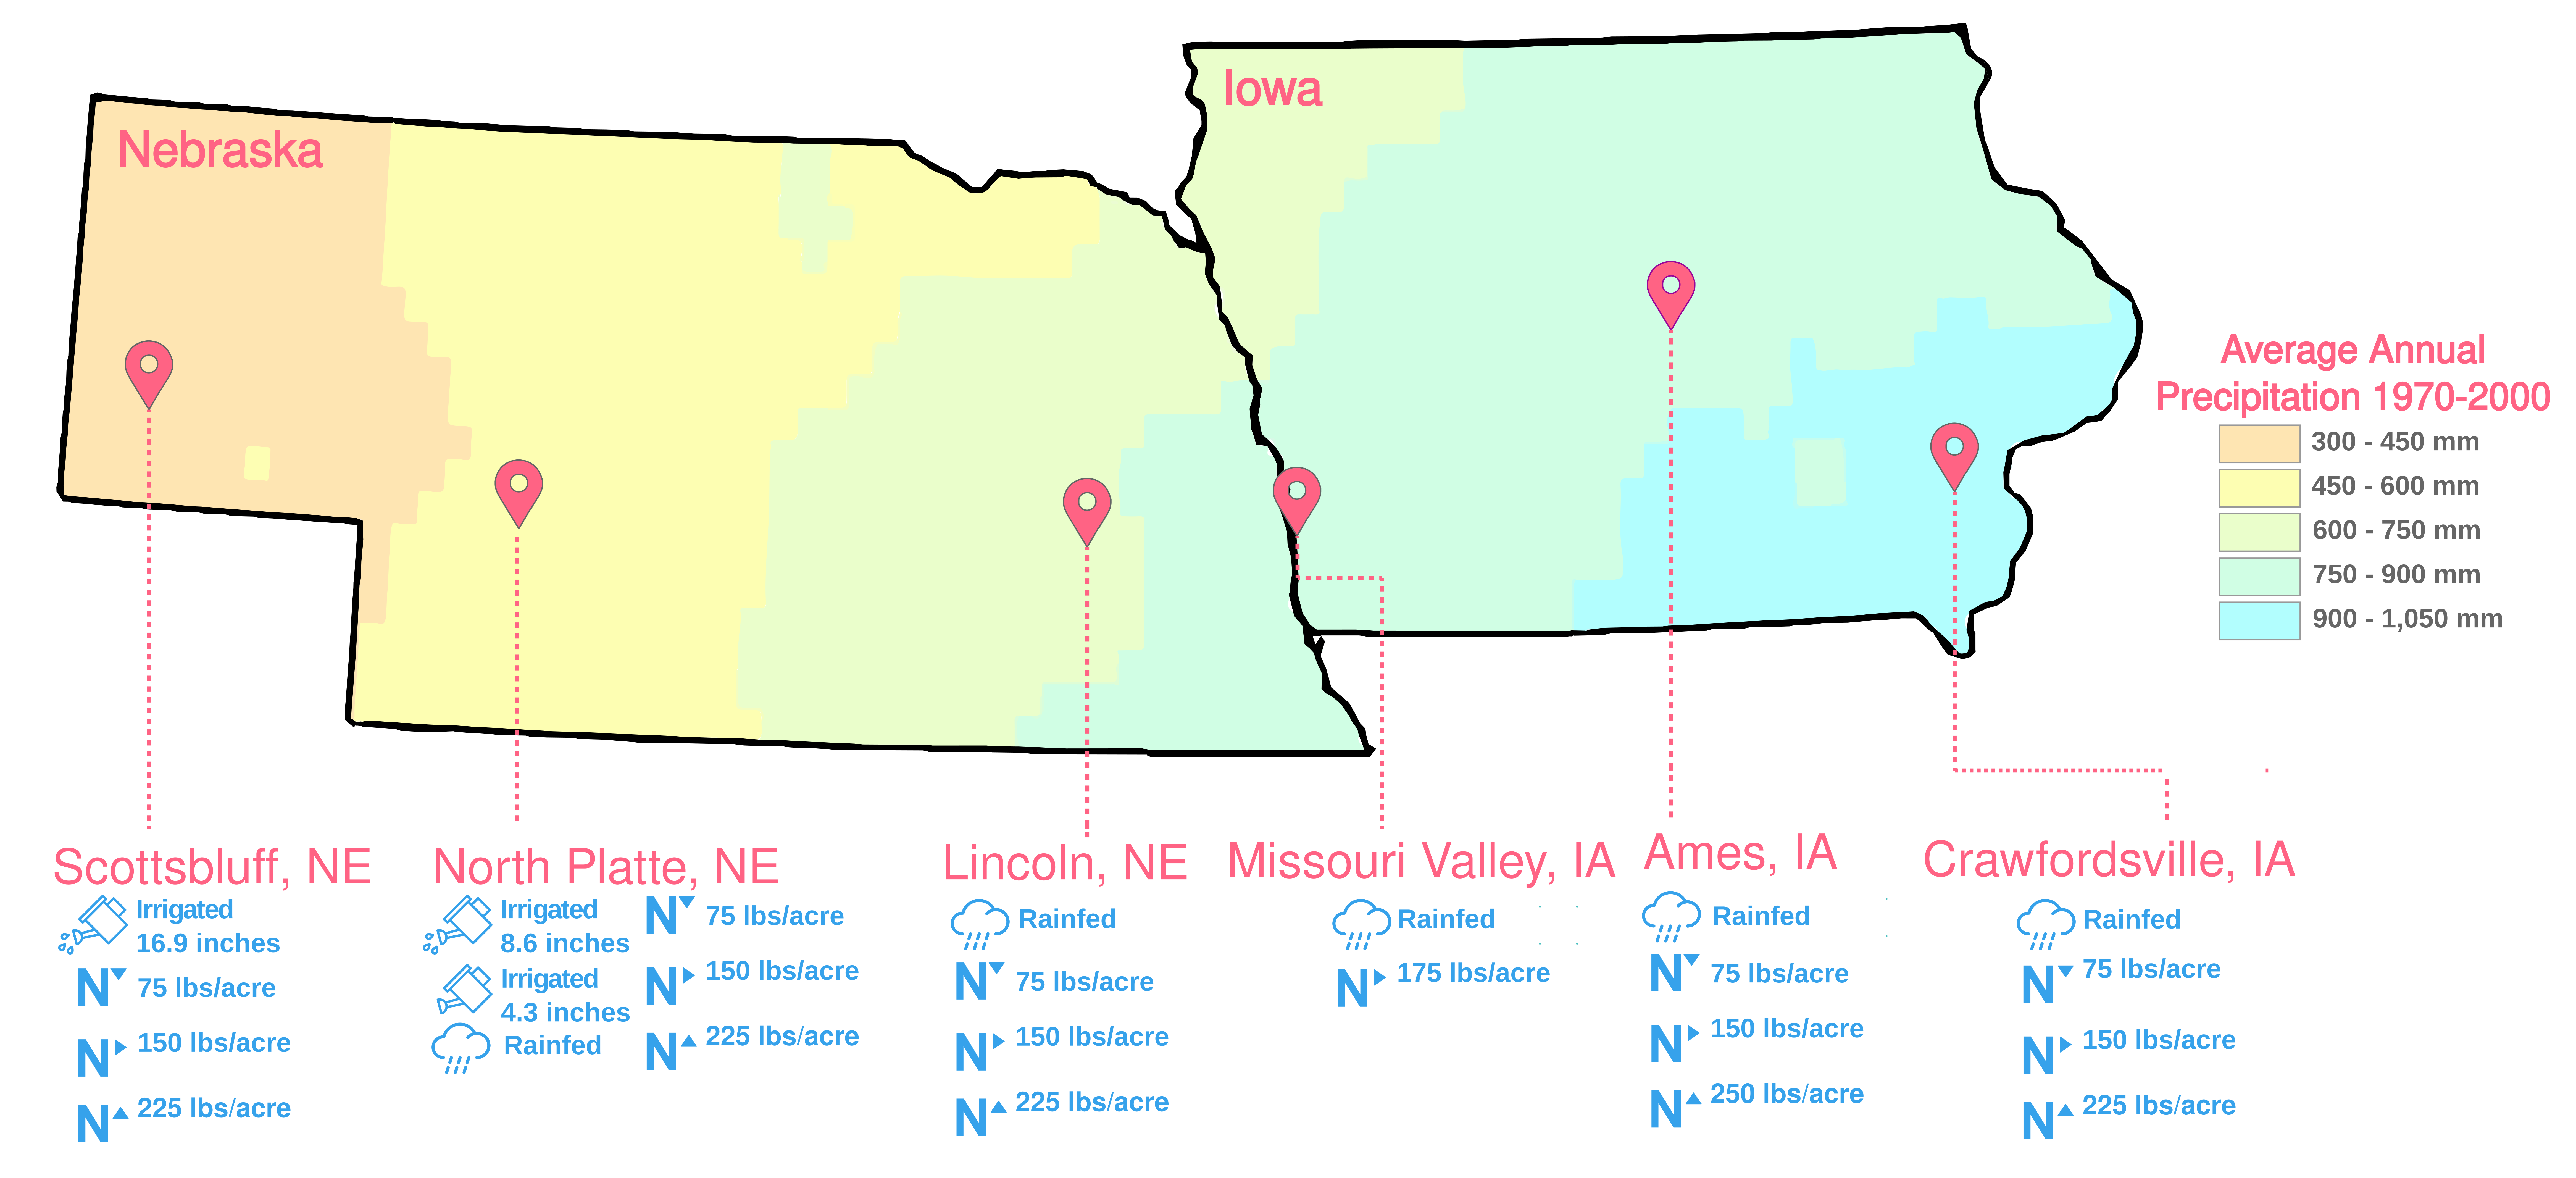
\includegraphics[width=1\linewidth]{MainFigures/Map.png}
    \caption{\textbf{Locations of six field experiments conducted across a rainfall gradient}. Scottsbluff and North Platte were irrigated; all other locations were rain-fed. With an exception of Missouri Valley, all other locations involved three levels of nitrogen fertilization.}
    \label{fig:locationoversview}
\end{figure}

\begin{figure}[h]
    \centering
    \includegraphics[width=0.8\linewidth]{MainFigures/FieldImage.png}
    \caption{\textbf{Overview of representative UAV and satellite images from Lincoln, deployment of ground control points (GCPs) and plot label segmentation} \textbf{A)} Orthomasaic UAV imagery of Lincoln field (top), cropped satellite image of Lincoln field (bottom). \textbf{B)} Cropped images showing ground control points (GCPs, inside red rectangle squares) installed at the corner of fields captured in UAV (left) and satellite image (right). \textbf{C)} Plot grids are generated across the field after assigning plot-level labels to field images.}
    \label{fig:plotsegment}
\end{figure}


\begin{figure}[h]
    \centering
    \includegraphics[width=0.98\linewidth]{MainFigures/Figure1.png}
    \caption{\textbf{Comparison between common features of satellite and UAV images captured within the same locations} \textbf{A)} Triangles indicate the dates at which UAV and satellite images were acquired. \textbf{B)} Correlation between the reflectance of the green band (\textit{$R_{green}$}) from Satellite and UAV images from two locations with the lowest temporal difference between satellite and UAV image acquisition at the first time point. The temporal difference between image acquisition of satellite and UAV was two days in Crawfordsville and 0 days in Missouri Valley. \textbf{C)} Correlation between \textit{$R_{green}$} of Satellite and UAV images and the temporal difference between satellite and UAV image acquisition within the same location. The numbers in the parenthesis in the legend correspond to the $R^2$ within each location. \textbf{D)} Correlation between the normalized difference green–red index (\textit{NGRDI}) of Satellite and UAV images and the temporal difference between satellite and UAV image acquisition within the same location. The numbers in the parenthesis in the legend correspond to the $R^2$ within each location. \textbf{E)} Example UAV RGB image from Scottsbluff field showing high spatial variability. \textbf{F)} Example UAV RGB image from Lincoln field showing variation between plots. 
    }
    \label{fig:Figure1}
\end{figure}


\begin{figure}[h]
    \centering
    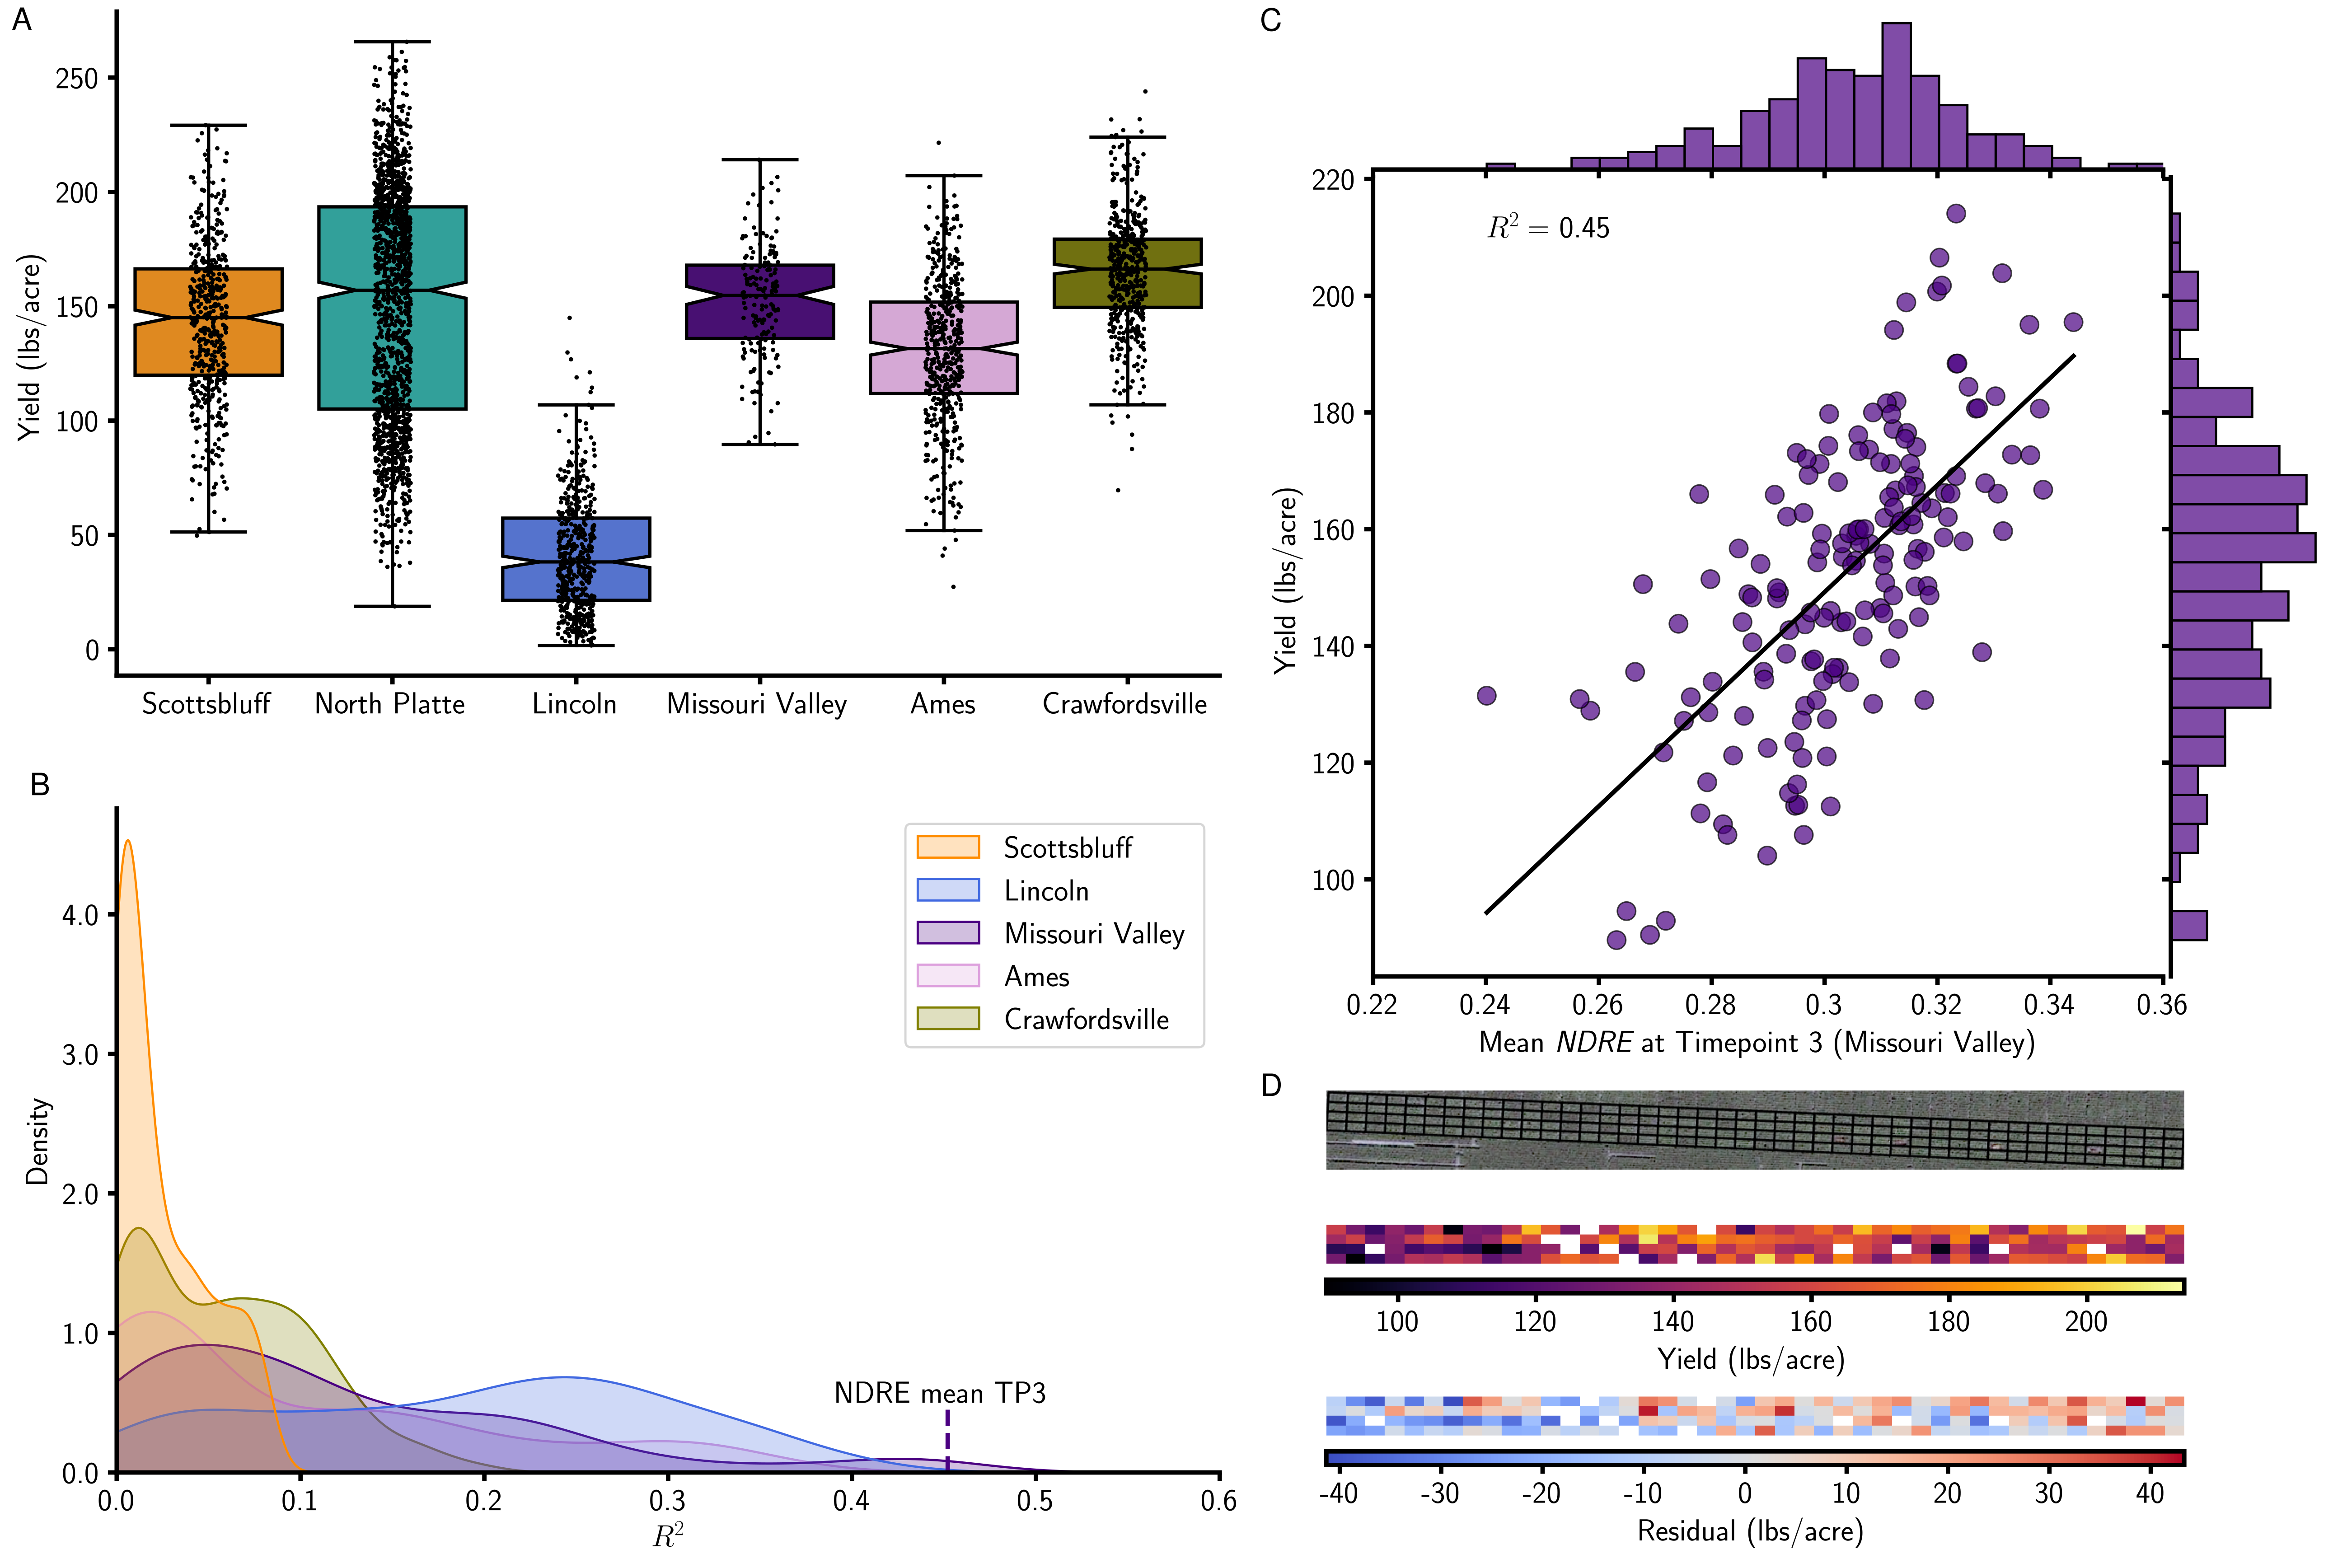
\includegraphics[width=1\linewidth]{MainFigures/Figure2.png}
    \caption{\textbf{Relationship of satellite image derived features with variation in yield across experimental locations} \textbf{A)} Box plots showing the variation in yield (lbs/acre) across field sites in Nebraska and Iowa. \textbf{B)} Density plot showing the distribution of $R^2$ values calculated between different features of plot-level images within the same location across different times of image acquisition with plot-level yield. The dashed vertical purple line represents the highest correlation ($R^2 = 0.45$) observed between the mean normalized difference red edge ($\textit{NDRE}$) in Missouri Valley at time point 3 (TP3, August 8, 2022) and yield per acre. \textbf{C)} Joint scatter and distribution plot showing the positive relationship between the highest correlated feature from Missouri Valley at TP3 (\textit{NDRE} mean TP3) from panel B and yield. \textbf{D)} Top; Field-level satellite image of the experimental field from Missouri Valley with plot grids generated during plot segmentation. Middle; yield map of plot level in Missouri Valley. Bottom; Residual map after yield prediction made on plot level from the highest correlated feature from panel C using the linear regression model (prediction of seen genotype in seen environment).}
    \label{fig:Figure2}
\end{figure}

\begin{figure}[h]
    \centering
    \includegraphics[width=0.6\linewidth]{MainFigures/Figure3.png}
    \caption{\textbf{Accuracy of yield prediction in different locations using satellite and UAV images acquired across the growing season.} \textbf{A)} Highest accuracy of yield prediction observed in Lincoln and Missouri Valley. Both prediction accuracies of two different locations and image types are shown based on the Random forest model using different image types acquired during the growing season; the color bar over the x-axis represents the growth stage recorded at Lincoln. The growth stage shown is for Lincoln. The second site at which flowering was scored, Scottsbluff, exhibited a similar date of peak flowering but a wider dispersion between the earliest and latest flowering lines. The error bar indicates the standard error (n=5) calculated from the prediction accuracy of five-fold cross-validation at each time point. Different colors represent different locations. The different line types represent the prediction accuracy of UAV and Satellite image types. In each fold, yield prediction is done for unseen genotypes in the seen environment. \textbf{B)} Heat map showing predictability of model trained on satellite images captured across different locations and times of the growing season. For each training data set, all the images from the location at that time point were used and testing was performed in the same location for all time points or in different locations at all time points. Yield prediction in this case was done for seen genotypes in both seen and unseen environments. X and Y axis color bars are based on different locations. The heat map color represents the model's prediction accuracy ($R^2$) comparing observed and predicted plot-level yield.
    }
    \label{fig:Figure3}
\end{figure}

\setcounter{table}{0}
\setcounter{figure}{0}
\renewcommand{\thetable}{S\arabic{table}}
\renewcommand{\thefigure}{S\arabic{figure}}

\begin{figure*}[h!]
\centering
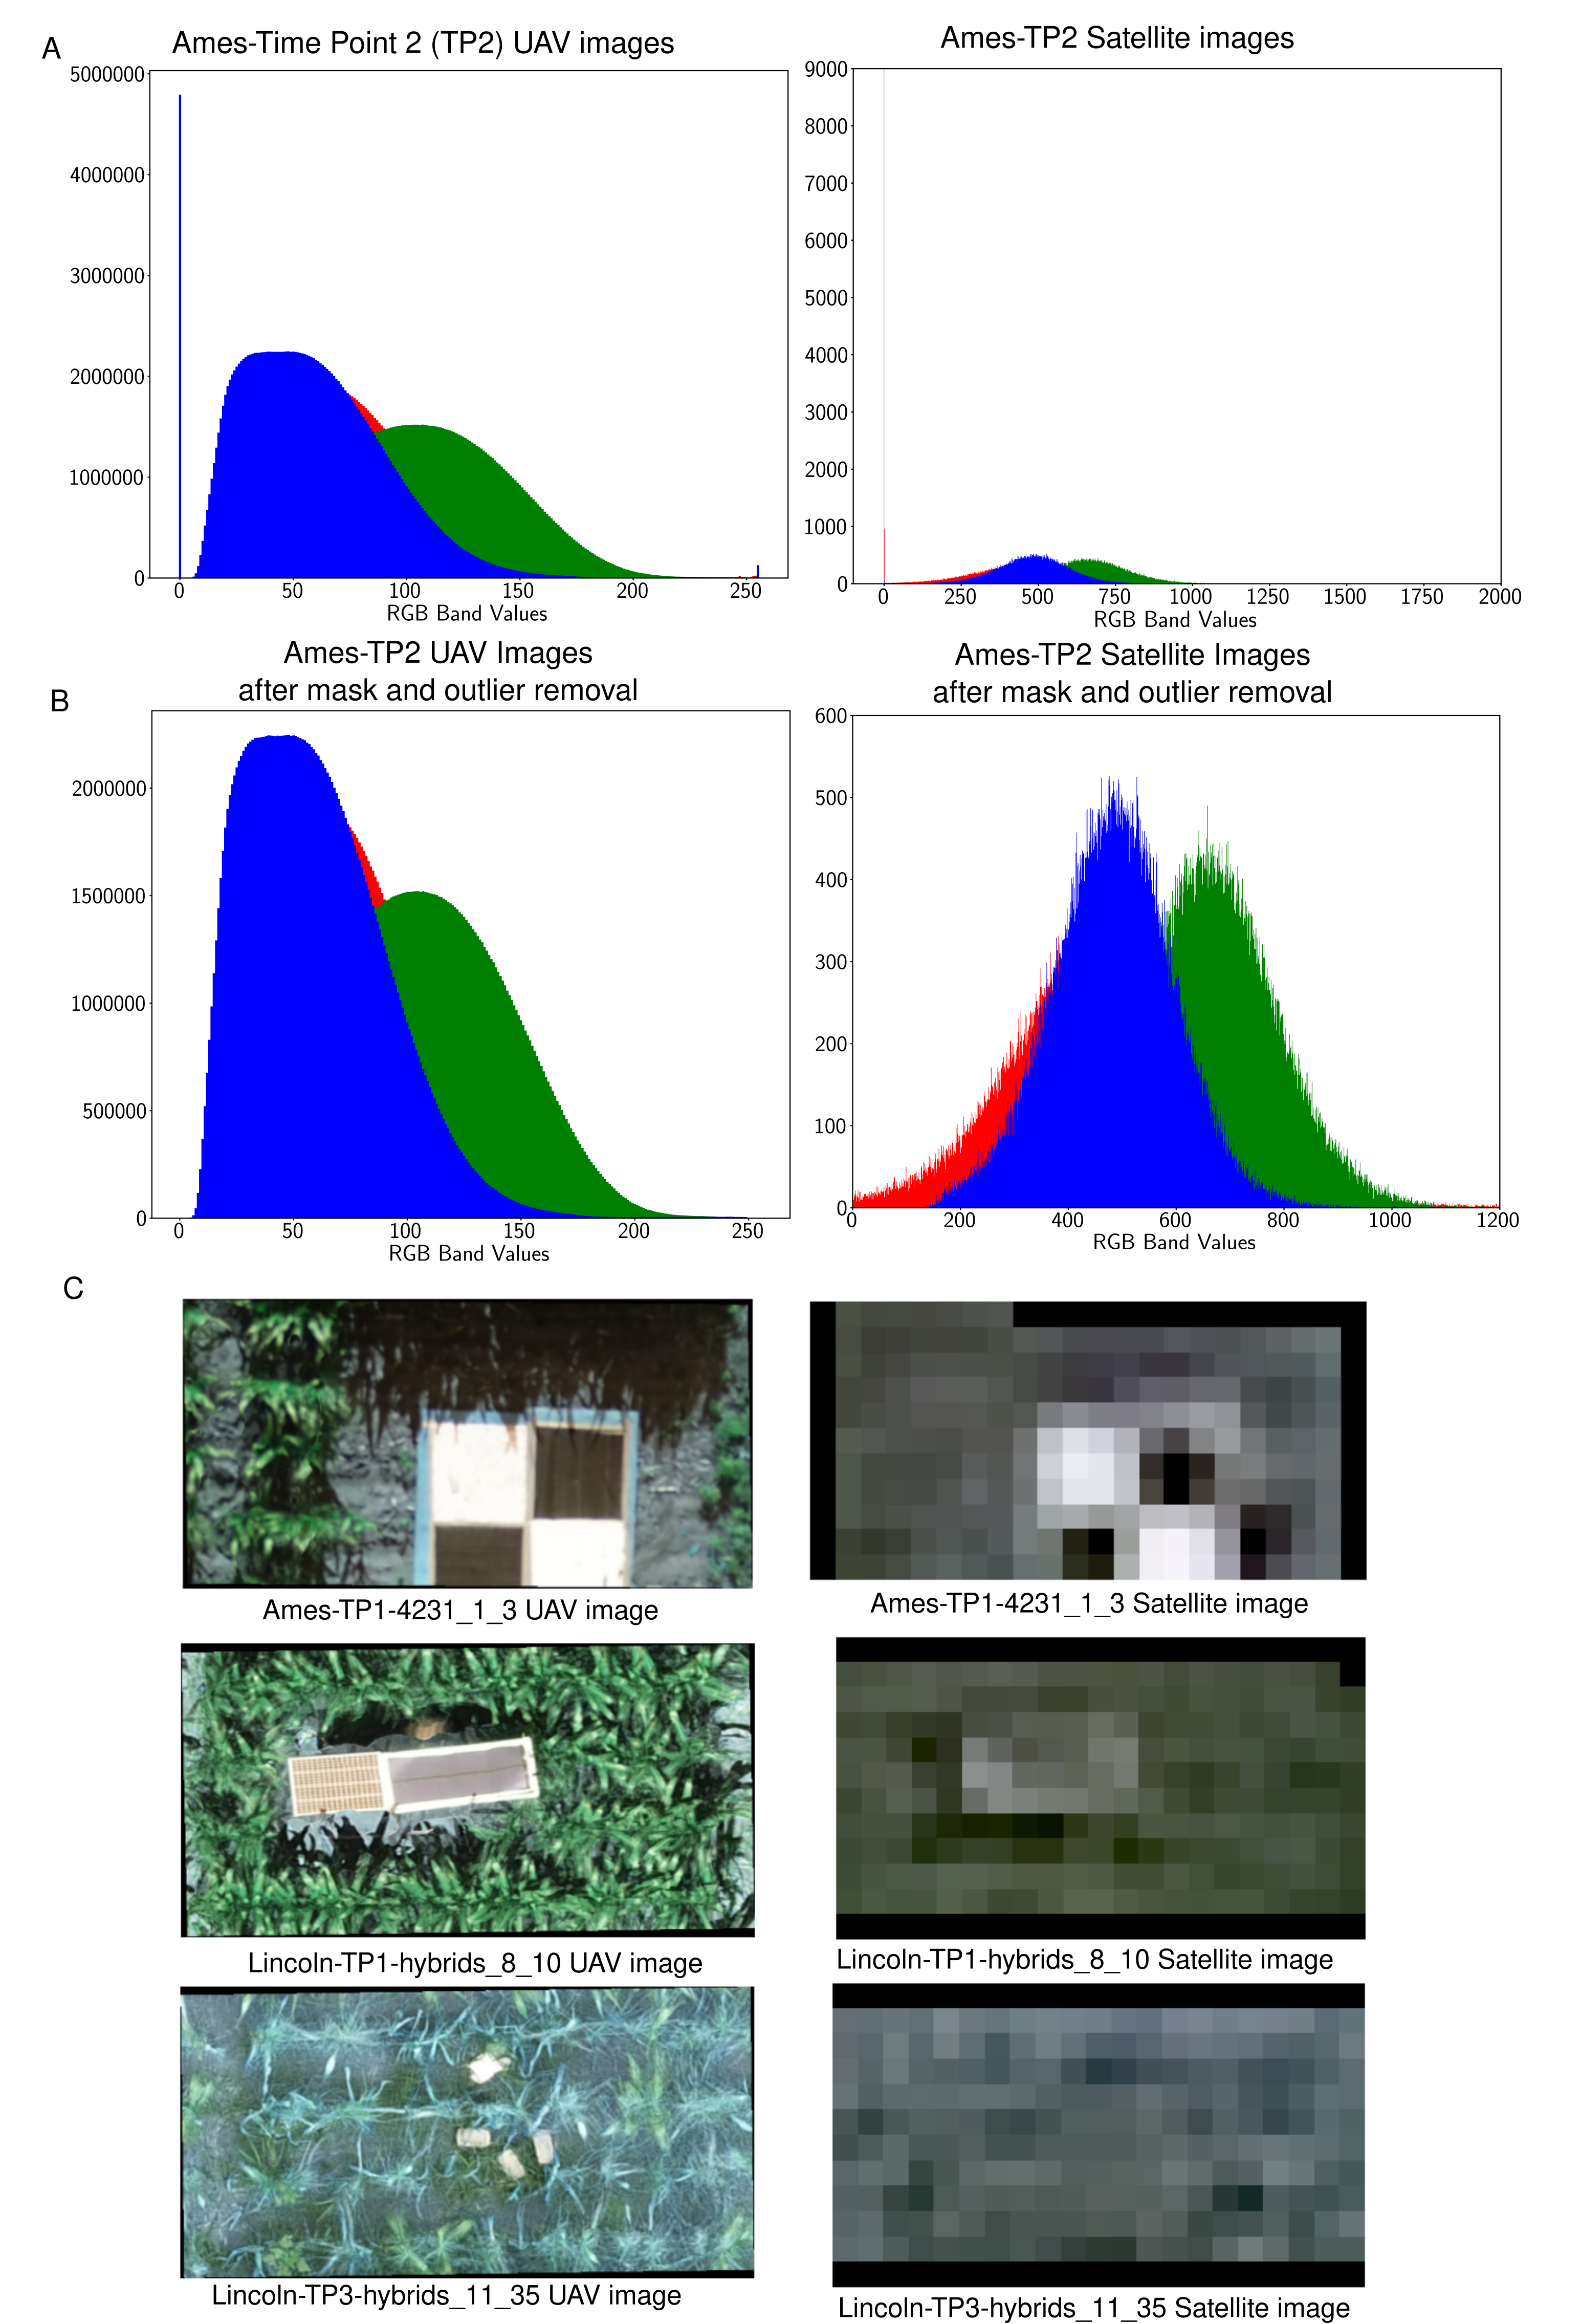
\includegraphics[width=0.7\textwidth]{SupplementalFigures/Supplementary1.png}
\caption{\textbf{Representative distribution plots of red, green, and blue bands} \textbf{A)} Distribution plot of red, green, and blue band values before the removal of mask and outliers in UAV (left) and satellite images (right) captured at Ames. \textbf{B)} Distribution plot of red, green, and blue band values after the removal of mask and outliers in UAV (left) and satellite images (right).
\textbf{C)} Example of UAV (left) and satellite (right) images from different locations to which outliers pixel values from the distribution plot were traced back.}
\label{fig:outlier}
\end{figure*}

\begin{figure*}[h!]
\centering
\includegraphics[width=0.7\textwidth]{SupplementalFigures/Figure_Ames.png}
\caption{\textbf{Representative UAV images of three field locations at Ames, Crawfordsville, and Missouri Valley.} The apparent spatial variability observed in Ames induced by shadows during flight was not observed in Crawfordsville and Missouri Valley.}
\label{fig:Ames}
\end{figure*}

% \setcounter{table}{0}
% \setcounter{figure}{0}
% \renewcommand{\thetable}{S\arabic{table}}
% \renewcommand{\thefigure}{S\arabic{figure}}
\begin{figure*}[h!]
\centering
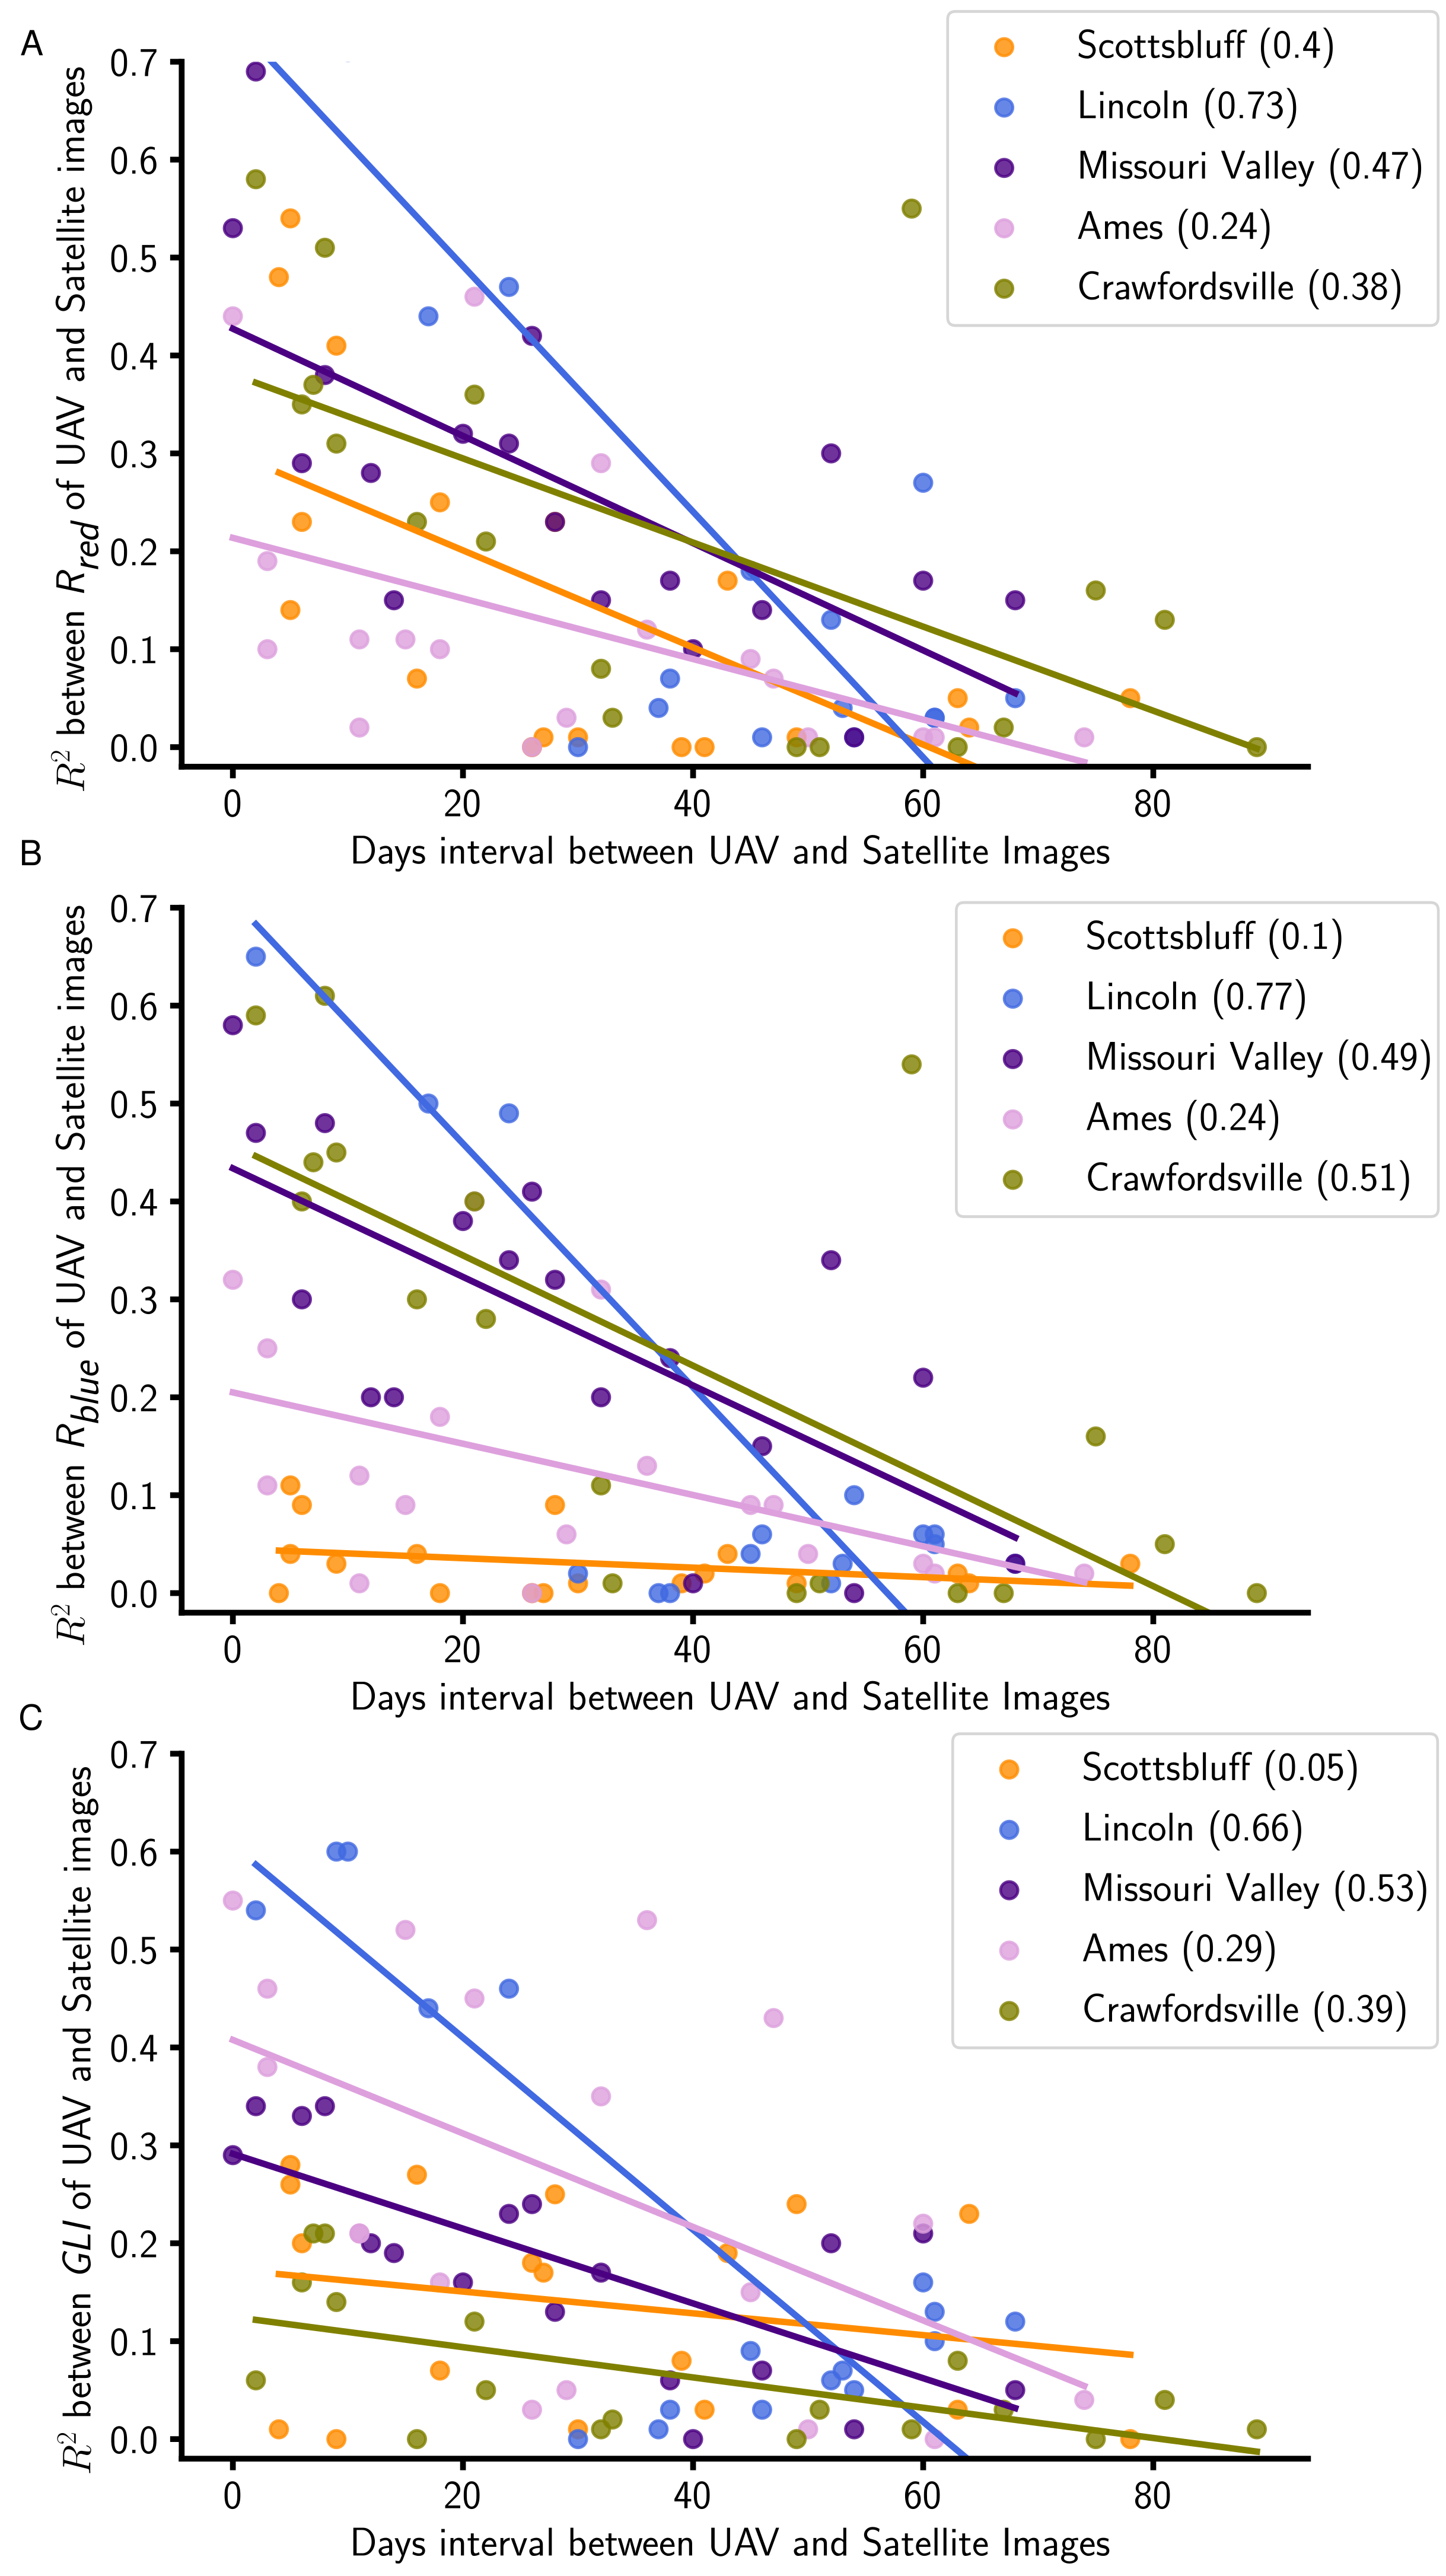
\includegraphics[width=0.6\textwidth]{SupplementalFigures/Figure1_supplementary.png}
\caption{\textbf{Correlations of common features between Satellite and UAV images decreases with increasing temporal difference.} Correlations ($R^2$) between \textbf{A)} $Reflectance_{green}$ ($R_{green}$), \textbf{B)} $Reflectance_{blue}$ ($R_{blue}$), and \textbf{C)} green leaf index ($GLI$) features derived from satellite and UAV images decrease as the temporal difference between satellite and UAV image acquisition increases. The numbers in the parenthesis in the key denote the $R^2$ within each location.
}
\label{fig:SatUAV_correlation}
\end{figure*}

\begin{figure*}[h!]
\centering
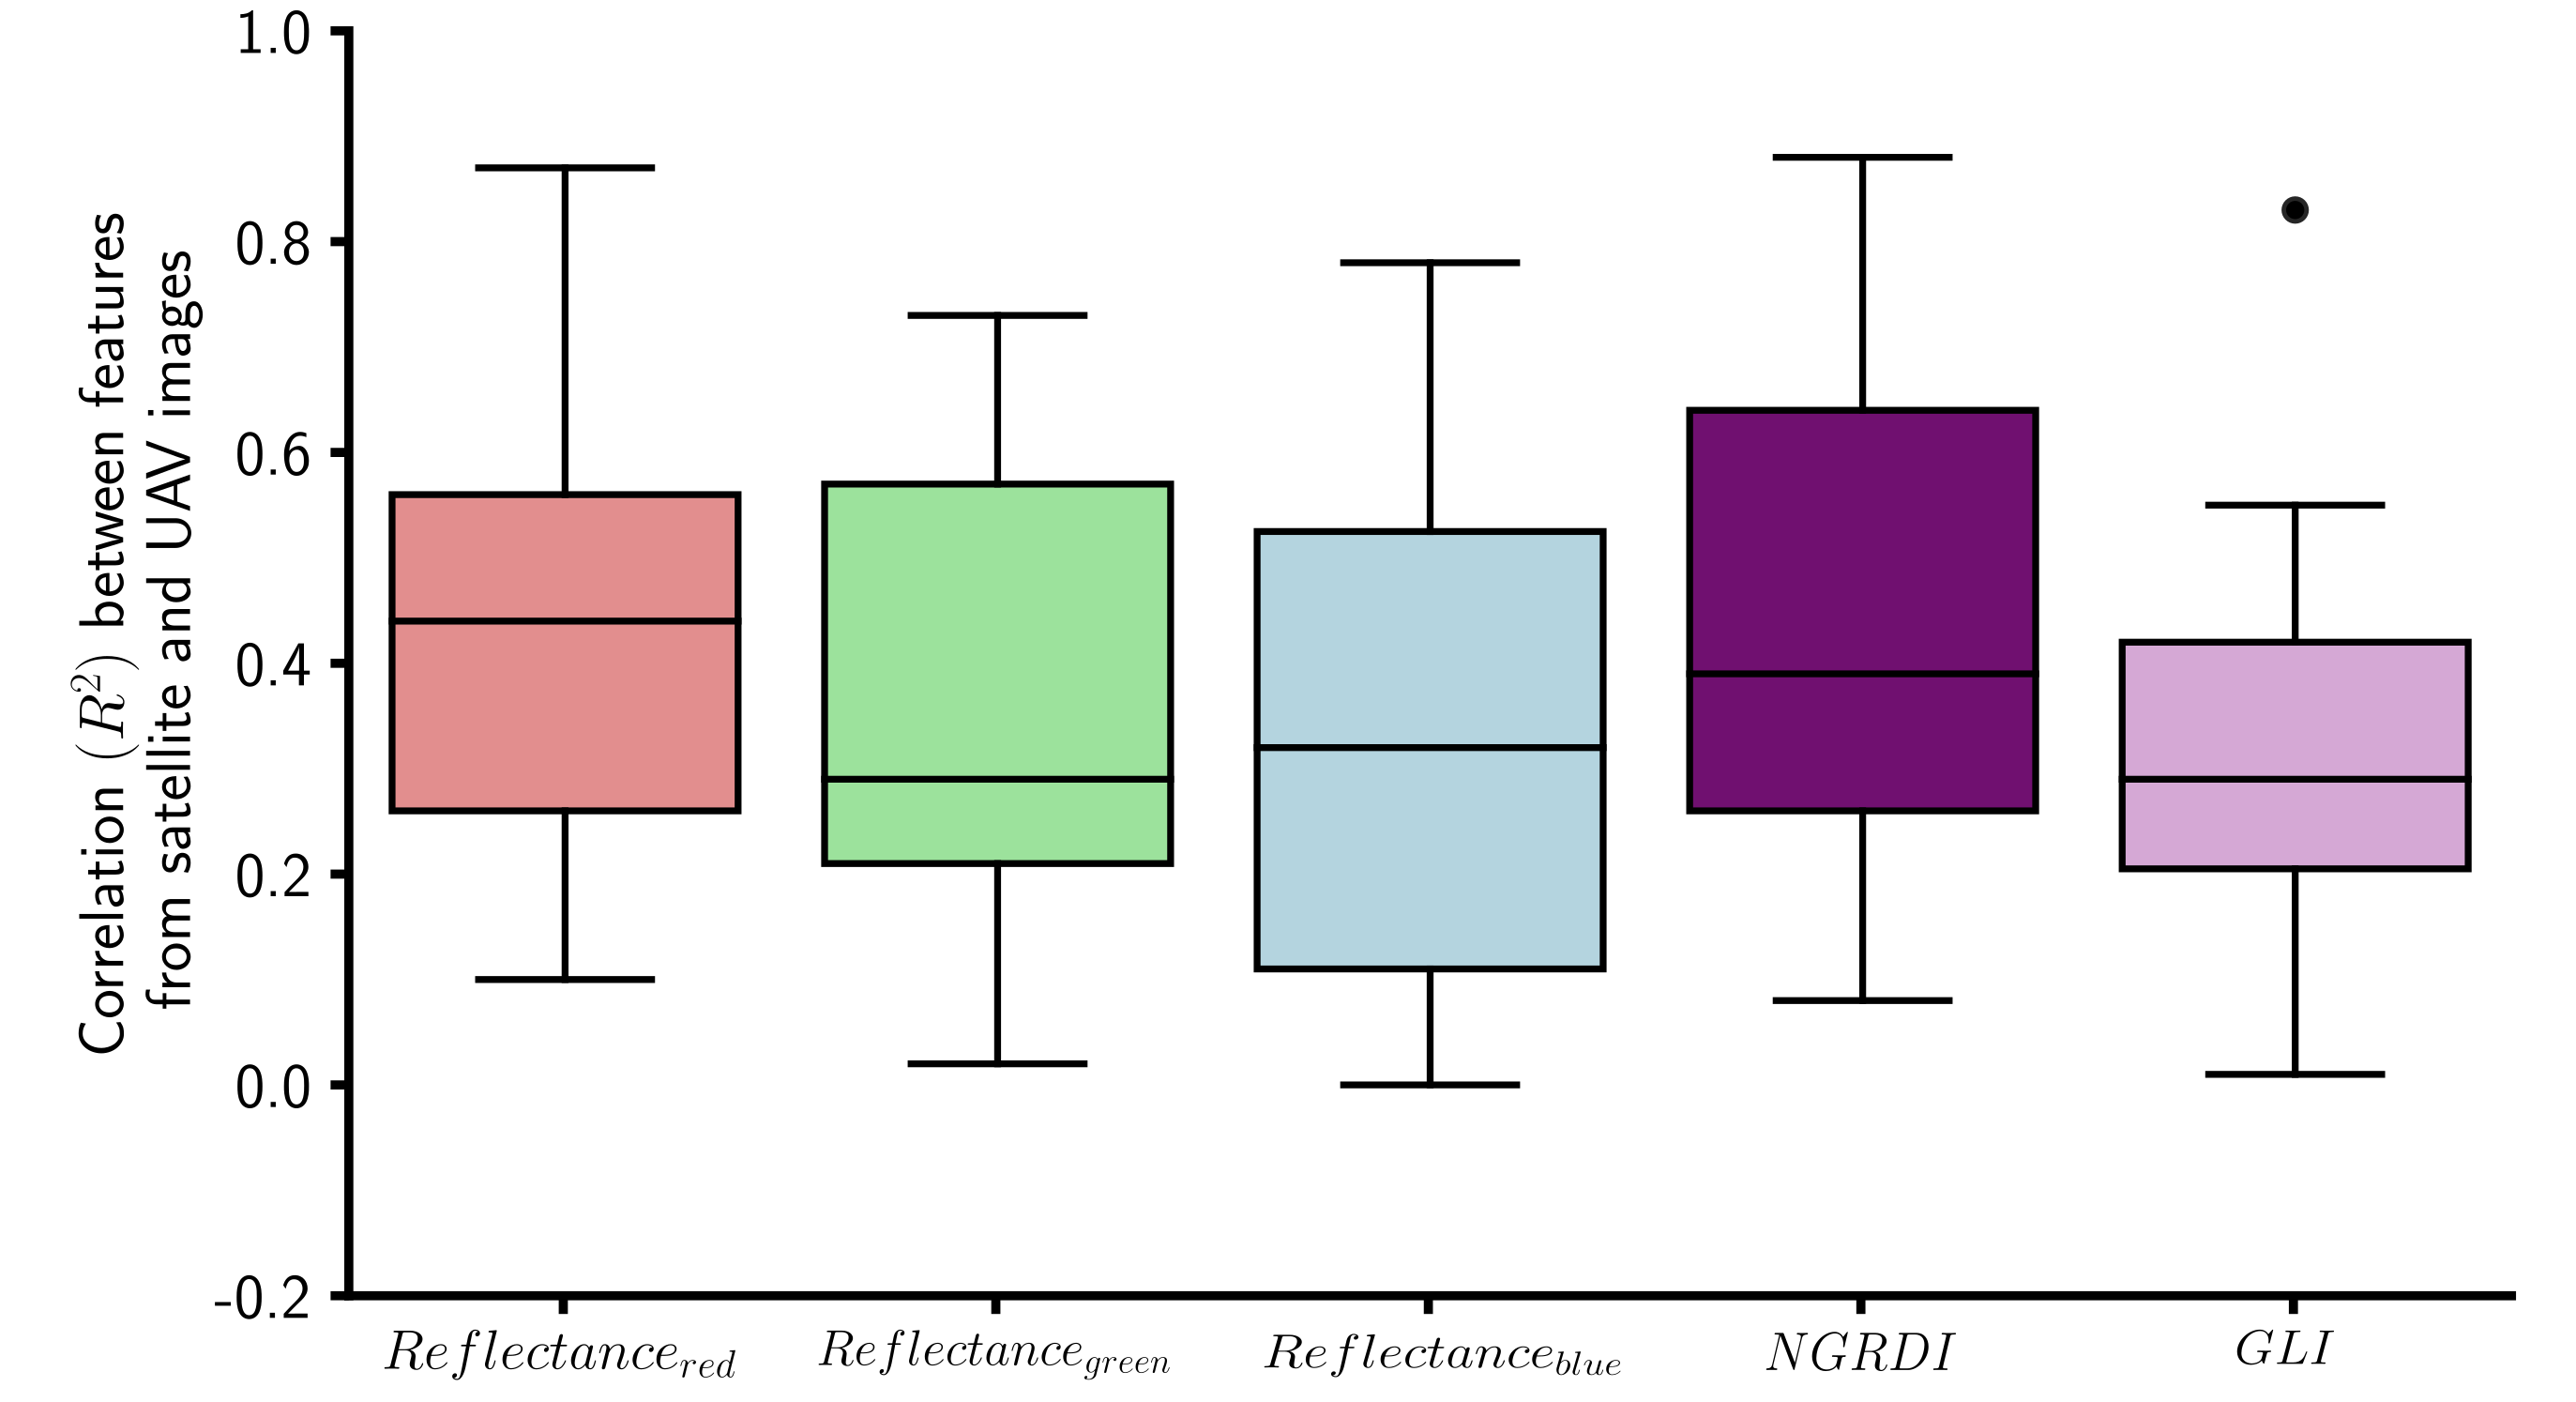
\includegraphics[width=1\textwidth]{SupplementalFigures/Figure1_corelation_supplemntary.png}
\caption{\textbf{Variation of $R^2$ observed between common mean features derived between Satellite and UAV images across all five locations with a temporal difference of at most one week between two image types} The number of observations (n) for each feature is 15 (n=15).
}
\label{fig:SatUAV_correlation_boxplot}
\end{figure*}


\begin{figure*}[h!]
\centering
\includegraphics[width=0.98\textwidth]{SupplementalFigures/SupplementaryRepCorrelation_allnitrogentoegther_nitrogen.png}
\caption{\textbf{Correlation between two replications of genotypes grown under the same treatment within the same location.} Different shades of green mapped to the scatter plot are based on three different nitrogen treatments employed across locations.}
\label{fig:yield_replication}
\end{figure*}

\begin{figure*}[h!]
\centering
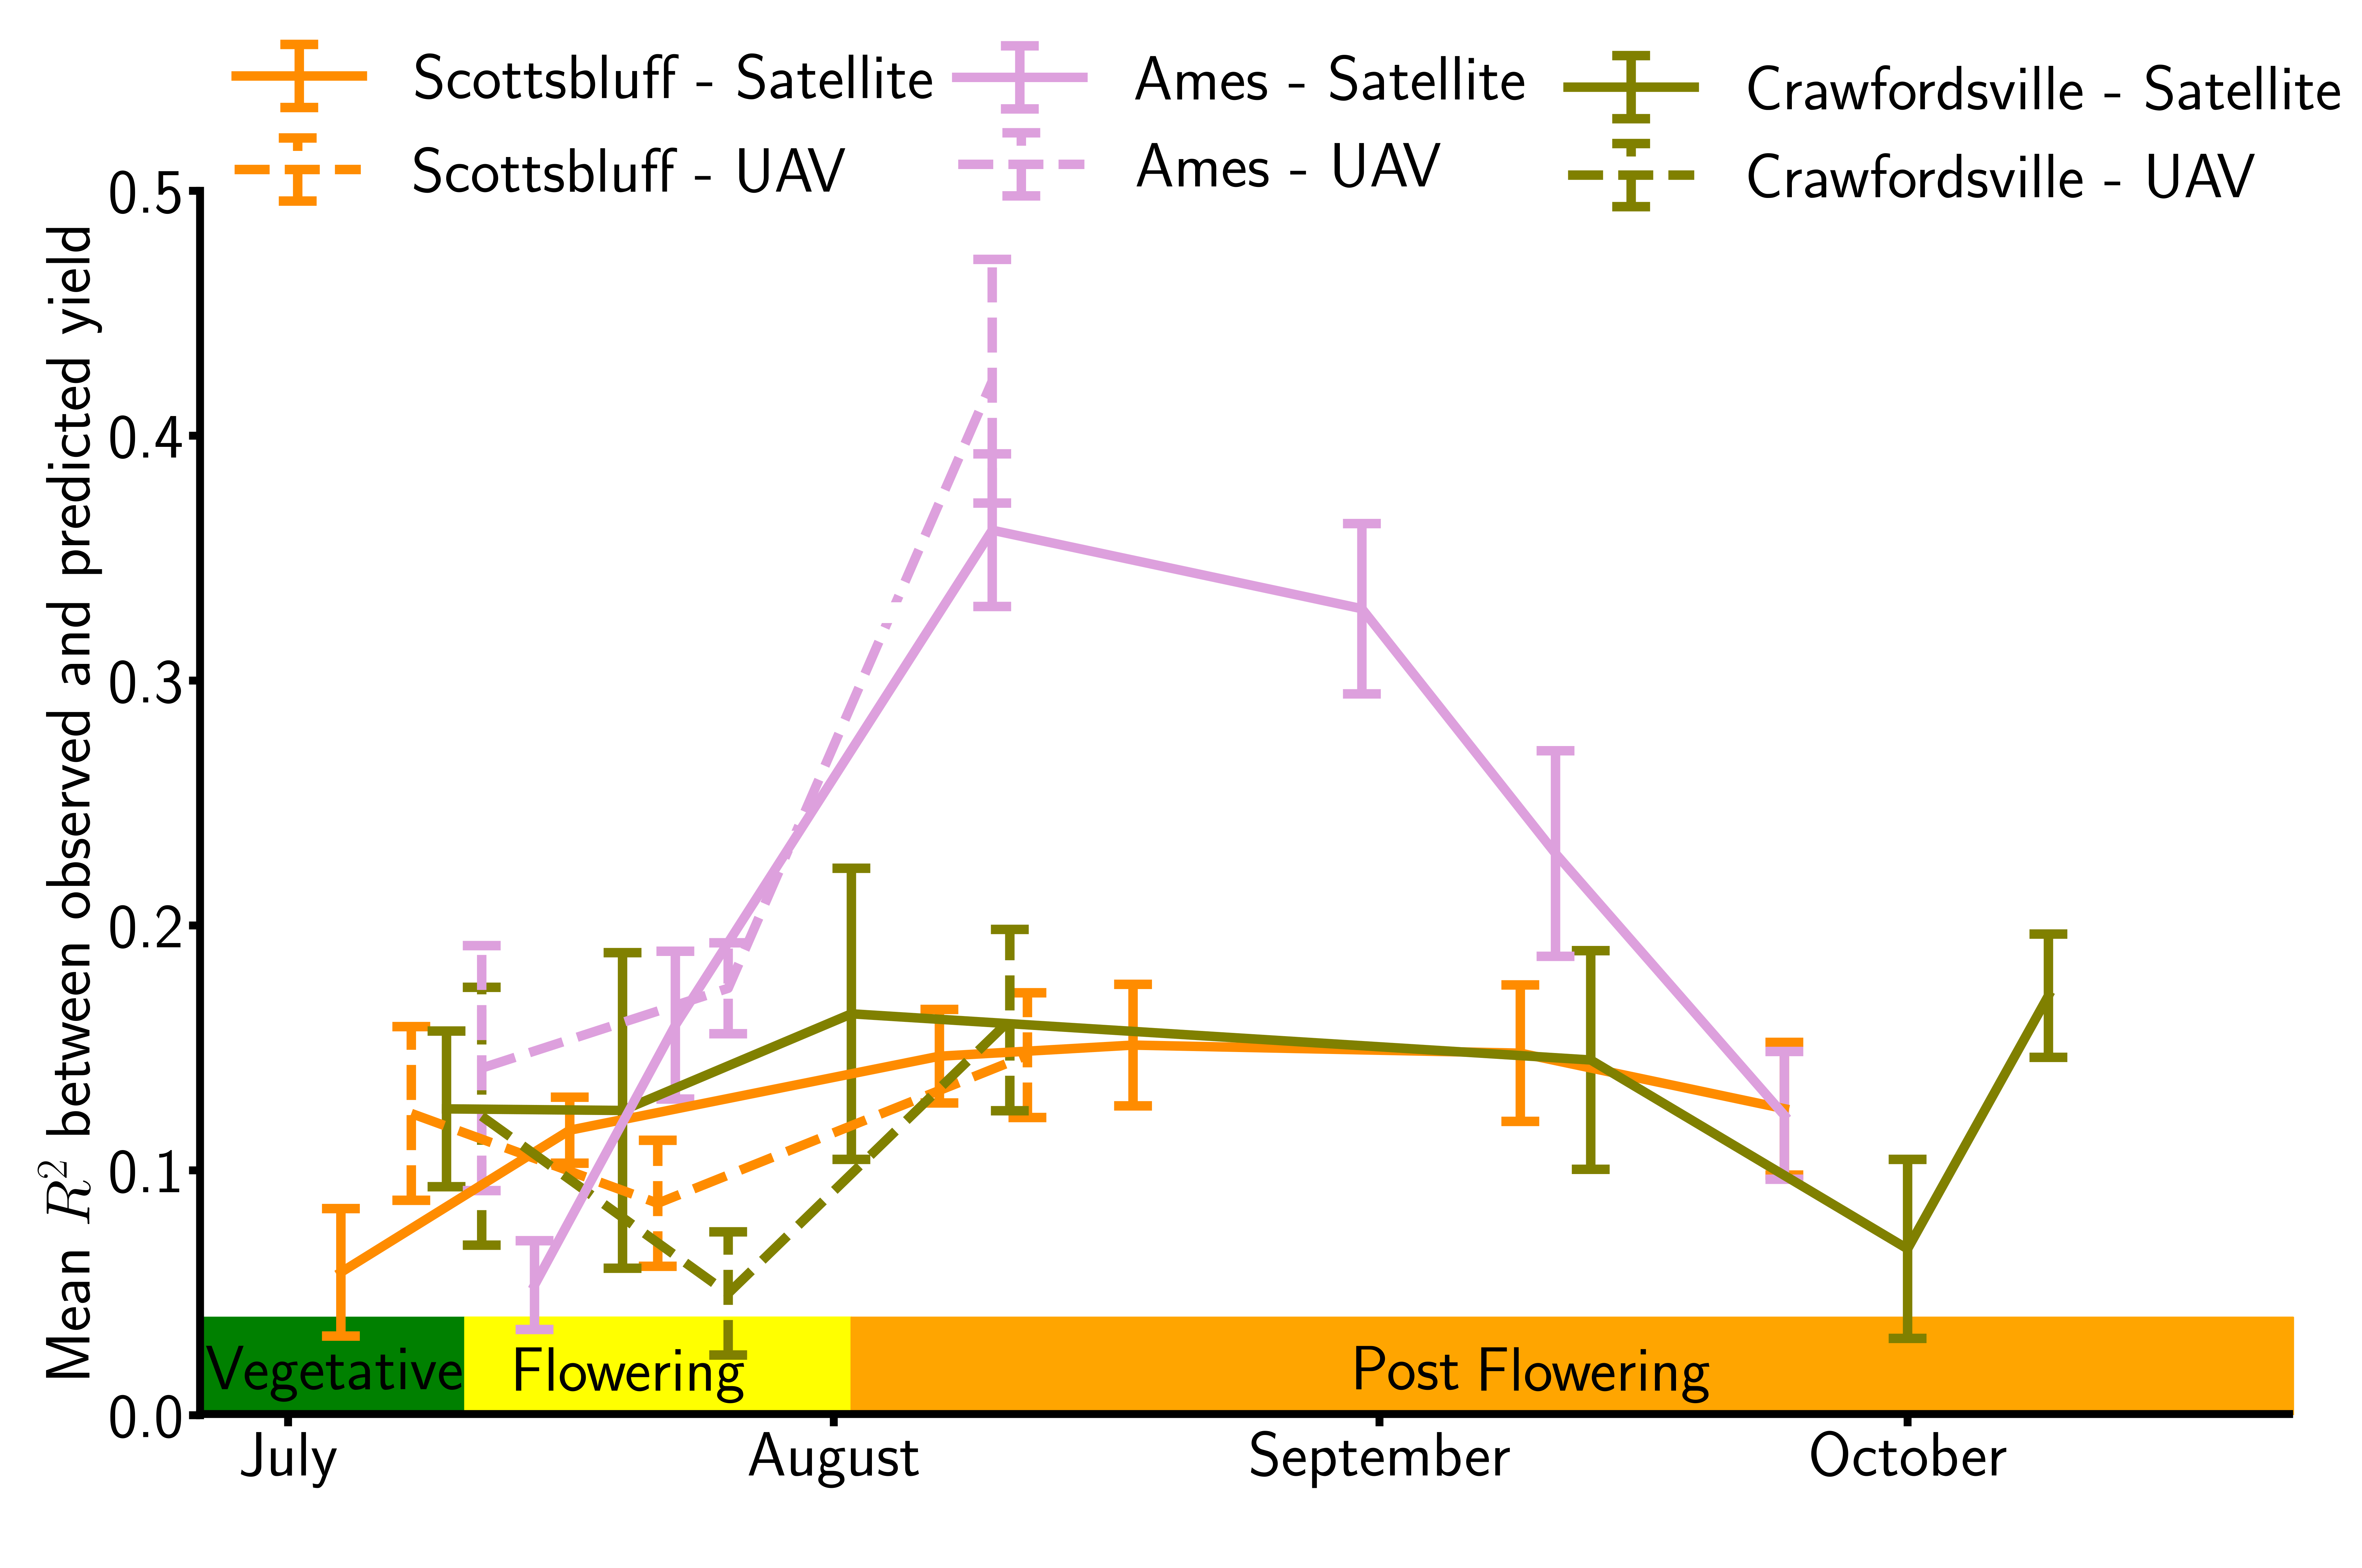
\includegraphics[width=0.98\textwidth]{SupplementalFigures/Figure3A_yield_supplementary.png}
\caption{\textbf{Performance of random forest model trained on satellite and UAV images to predict yield in Scottsbluff, Ames, and Crawfordsville.} Different line types correspond to model performance based on either satellite or UAV images. Different line colors correspond to model performance for predicting plot level yield of unseen genotypes in a seen environment in terms of $R^2$ between observed and predicted plot level yield within 5-fold cross-validation. The error bar represents standard error from 5-fold cross-validation (n=5). The coloring for different growth stages above the x-axis is done based on the dates recorded at the Lincoln field experiment.The second site at which flowering was scored, Scottsbluff, exhibited a similar date of peak flowering but a wider dispersion between the earliest and latest flowering lines.}
\label{fig:modelperformance_supplementary}
\end{figure*}

\begin{figure*}[h!]
\centering
\includegraphics[width=0.7\textwidth]{SupplementalFigures/Figure3_totalstandcount_rf.png}
\caption{\textbf{ Model performance to predict total stand count in three locations where we had ground truth data} \textbf{A).} Performance of random forest model trained on satellite and UAV images to predict total stand count in Missouri Valley, Ames, and Crawfordsville. Different line types correspond to model performance based on either satellite or UAV images. Different line colors correspond to model performance for predicting plot level yield of unseen genotypes in a seen environment in terms of $R^2$ between observed and predicted plot level yield within 5-fold cross-validation. The error bar represents standard error from 5-fold cross-validation (n=5). The coloring for different growth stages above the x-axis is done based on the dates recorded at the Lincoln field experiment.
\textbf{B).} Heat map showing predictability of model to estimate total stand count trained on satellite images captured across different locations and times of the growing season. The training is performed with the same approach as in Figure~\ref{fig:Figure3}B.
}
\label{fig:totalstandcount}
\end{figure*}


\begin{figure*}[h!]
\centering
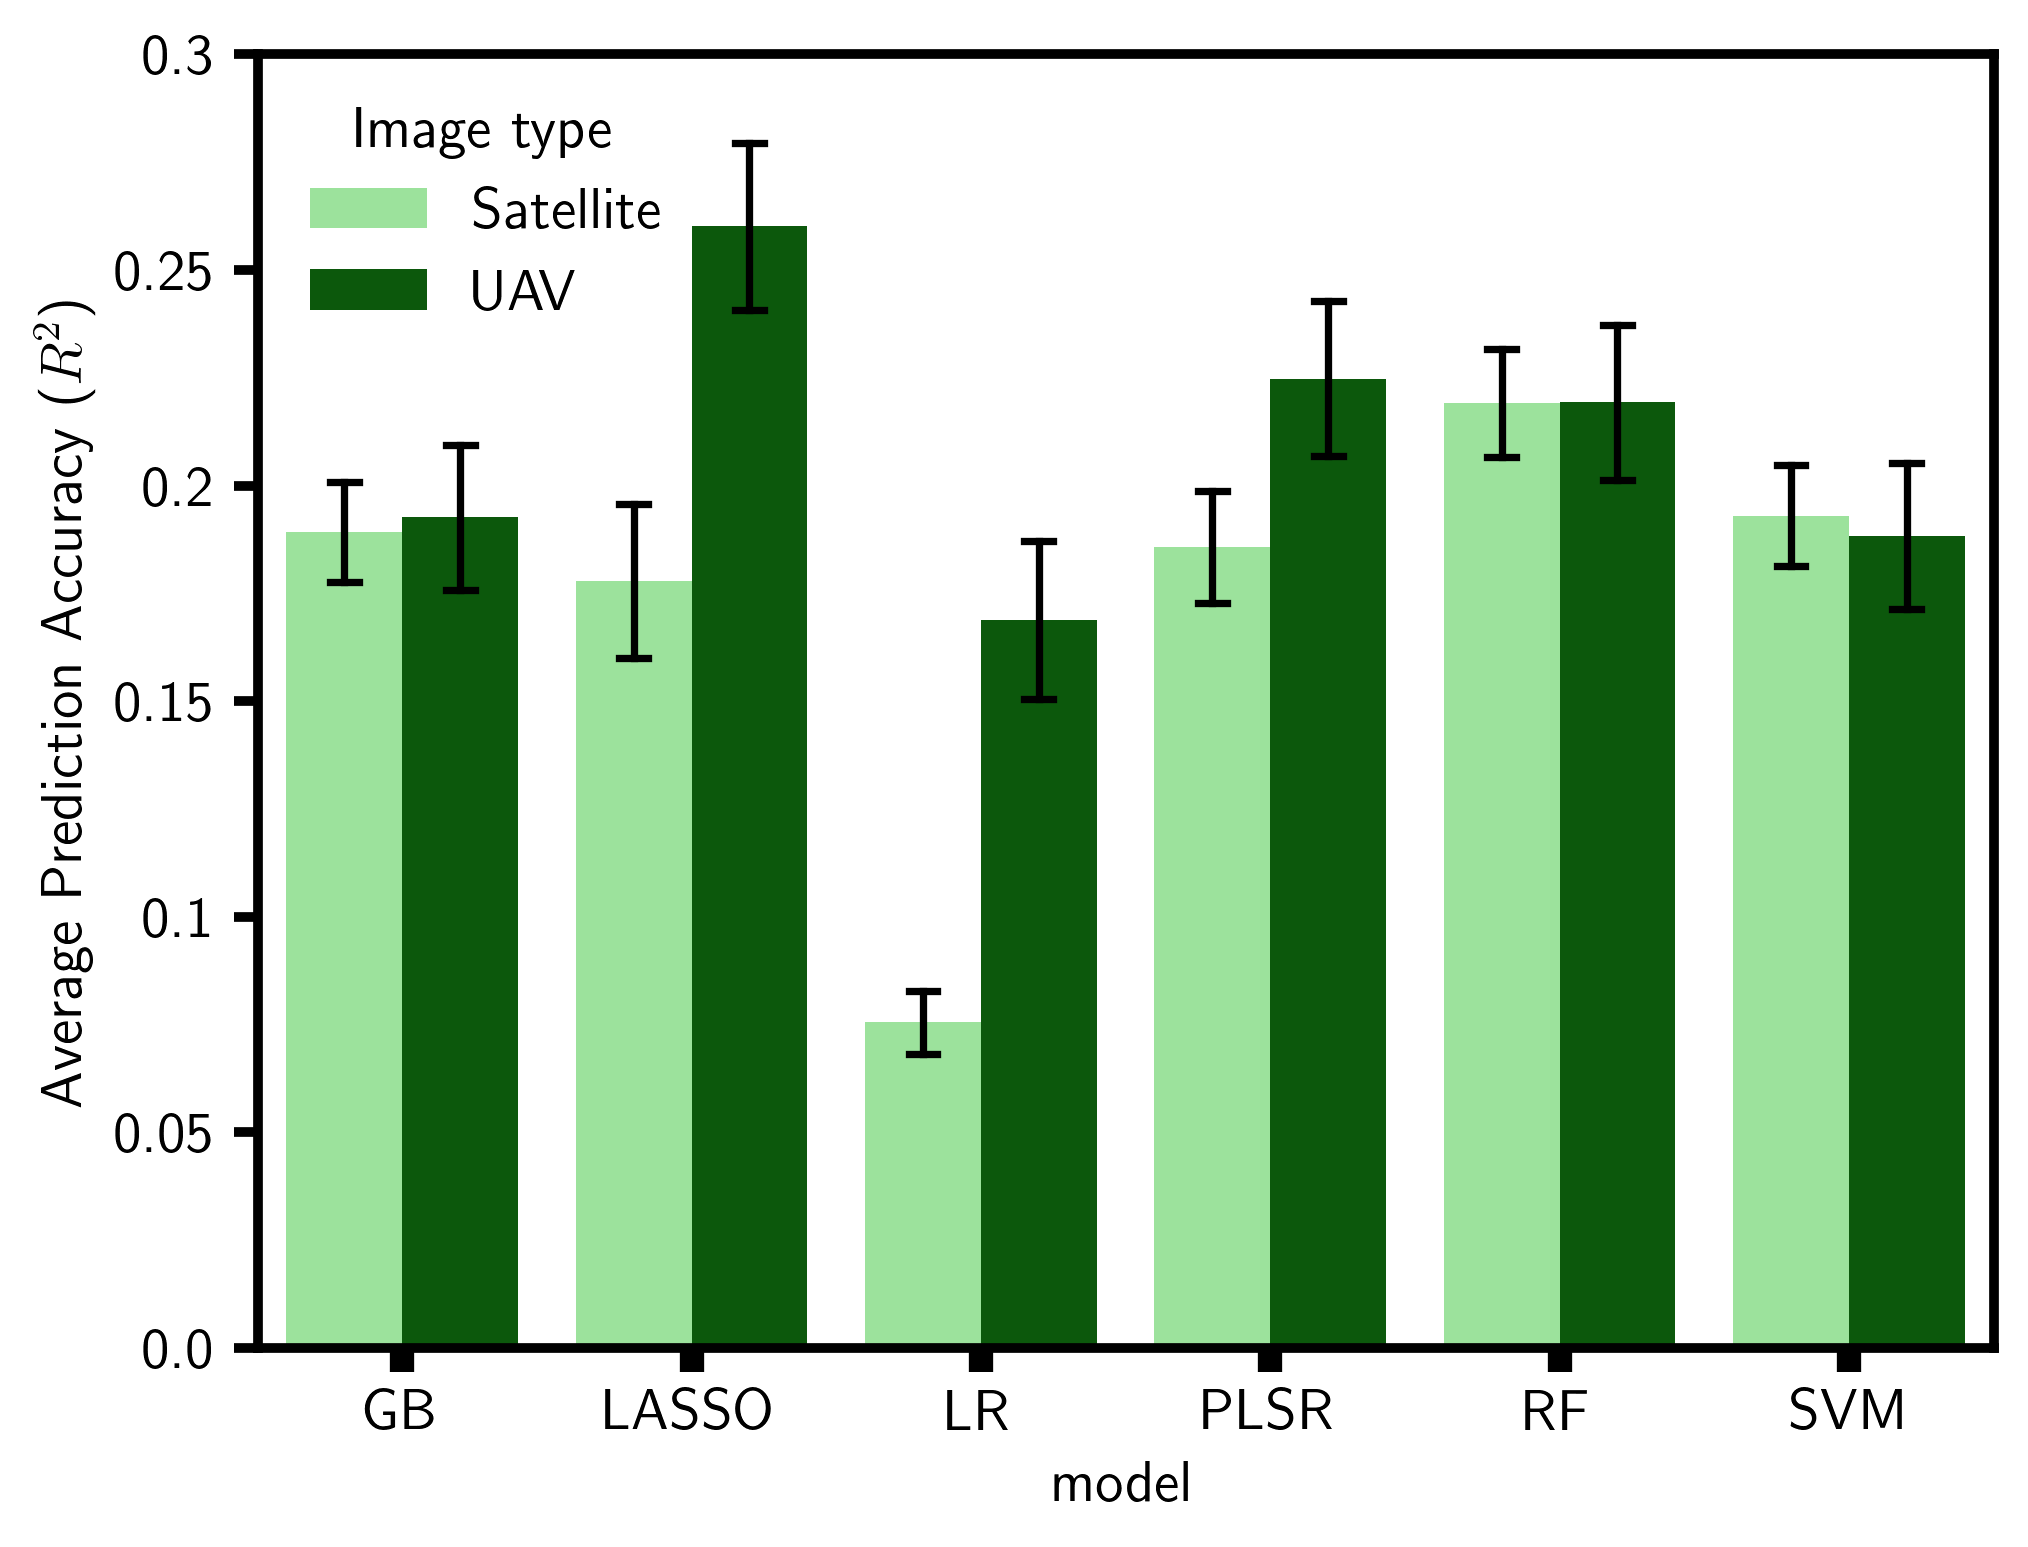
\includegraphics[width=0.50\textwidth]{SupplementalFigures/AverageAcc_Models.png}
\caption{\textbf{Average performance of different machine learning tools used in the study across different locations and time points using satellite and UAV images.} Evaluated models include gradient boost (GB), Least Absolute Shrinkage and Selection Operator (LASSO), Linear Regression (LR), Partial least squares regression (PLSR), Random forest (RF), and Support vector machine (SVM). Each model was trained on features derived from satellite and UAV images separately. The LASSO model did not converge in the case of some satellite and UAV images.
The error bar represents the standard error for each model across different locations and time points.}
\label{fig:averagemodelperformance}
\end{figure*}


\begin{figure*}[h!]
\centering
\includegraphics[width=0.98\textwidth]{SupplementalFigures/Fiigure3B_yieldperacre_UAV.png}
\caption{\textbf{Predictability of random forest model trained on UAV images to predict the yield of genotypes in unseen environments.} Heat map showing predictability of model to estimate yield trained on UAV images
captured across different locations and times of the growing season. The training is performed with the same approach as in Figure~\ref{fig:Figure3}B.
}
\label{fig:modelperformanceUAV}
\end{figure*}




\newpage
\bibliography{example-bibliography}
% \bibliography{example-bibliography}
\end{document}Translational AI Research and Education Center,